\documentclass[10pt]{beamer}\usepackage[]{graphicx}\usepackage[]{color}
% maxwidth is the original width if it is less than linewidth
% otherwise use linewidth (to make sure the graphics do not exceed the margin)
\makeatletter
\def\maxwidth{ %
  \ifdim\Gin@nat@width>\linewidth
    \linewidth
  \else
    \Gin@nat@width
  \fi
}
\makeatother

\definecolor{fgcolor}{rgb}{0.345, 0.345, 0.345}
\newcommand{\hlnum}[1]{\textcolor[rgb]{0.686,0.059,0.569}{#1}}%
\newcommand{\hlstr}[1]{\textcolor[rgb]{0.192,0.494,0.8}{#1}}%
\newcommand{\hlcom}[1]{\textcolor[rgb]{0.678,0.584,0.686}{\textit{#1}}}%
\newcommand{\hlopt}[1]{\textcolor[rgb]{0,0,0}{#1}}%
\newcommand{\hlstd}[1]{\textcolor[rgb]{0.345,0.345,0.345}{#1}}%
\newcommand{\hlkwa}[1]{\textcolor[rgb]{0.161,0.373,0.58}{\textbf{#1}}}%
\newcommand{\hlkwb}[1]{\textcolor[rgb]{0.69,0.353,0.396}{#1}}%
\newcommand{\hlkwc}[1]{\textcolor[rgb]{0.333,0.667,0.333}{#1}}%
\newcommand{\hlkwd}[1]{\textcolor[rgb]{0.737,0.353,0.396}{\textbf{#1}}}%
\let\hlipl\hlkwb

\usepackage{framed}
\makeatletter
\newenvironment{kframe}{%
 \def\at@end@of@kframe{}%
 \ifinner\ifhmode%
  \def\at@end@of@kframe{\end{minipage}}%
  \begin{minipage}{\columnwidth}%
 \fi\fi%
 \def\FrameCommand##1{\hskip\@totalleftmargin \hskip-\fboxsep
 \colorbox{shadecolor}{##1}\hskip-\fboxsep
     % There is no \\@totalrightmargin, so:
     \hskip-\linewidth \hskip-\@totalleftmargin \hskip\columnwidth}%
 \MakeFramed {\advance\hsize-\width
   \@totalleftmargin\z@ \linewidth\hsize
   \@setminipage}}%
 {\par\unskip\endMakeFramed%
 \at@end@of@kframe}
\makeatother

\definecolor{shadecolor}{rgb}{.97, .97, .97}
\definecolor{messagecolor}{rgb}{0, 0, 0}
\definecolor{warningcolor}{rgb}{1, 0, 1}
\definecolor{errorcolor}{rgb}{1, 0, 0}
\newenvironment{knitrout}{}{} % an empty environment to be redefined in TeX

\usepackage{alltt}


%\input{slides_header.tex}
\usepackage{graphicx}
\usepackage{hyperref, url}
\hypersetup{colorlinks,citecolor=myorange,filecolor=red,linkcolor=brown,urlcolor=blue}

\usepackage{longtable,booktabs}
\usepackage{amssymb,amsmath}
\usepackage{animate}
\usepackage{subfig}
\usepackage{tikz}
\usetikzlibrary{shapes.geometric, arrows,shapes.symbols,decorations.pathreplacing}
\tikzstyle{startstop} = [rectangle, rounded corners, minimum width=3cm, minimum height=1cm, draw=black, fill=pinkish,text width=3.5cm]
\tikzstyle{startstop2} = [rectangle, rounded corners, minimum width=3cm, minimum height=1cm, draw=black, fill=background,text width=4.5cm]
\tikzstyle{startstop3} = [rectangle, rounded corners, minimum width=3cm, minimum height=1cm, draw=black, fill=beige,text width=3.0cm]
\tikzstyle{startstop4} = [rectangle, rounded corners, minimum width=3cm, minimum height=1cm, draw=black, fill=pinkish,text width=4.5cm]
\tikzstyle{io} = [trapezium, trapezium left angle=70, trapezium right angle=110, minimum width=2cm, minimum height=1cm, text centered, draw=black, fill=blue!30,text width=1.5cm]
\tikzstyle{process} = [rectangle, minimum width=1cm, minimum height=1cm, text centered, draw=black, fill=orange!30,text width=2cm]
\tikzstyle{decision} = [diamond, minimum width=2cm, minimum height=1cm, text centered, draw=black, fill=green!30]
\tikzstyle{arrow} = [thick,->,>=stealth]
\tikzstyle{both} = [thick,<->,>=stealth, red]


% used for tree of stats tests in 001-introduction
\tikzstyle{startstopstats} = [rectangle, rounded corners, minimum width=2cm, minimum height=.5cm,text centered, draw=black, fill=red!30]
\tikzstyle{iostats} = [trapezium, trapezium left angle=70, trapezium right angle=110, minimum width=2cm, minimum height=.5cm, text centered, draw=black, fill=blue!30]
\tikzstyle{processstats} = [rectangle, minimum width=1.5cm, minimum height=.5cm, text centered, draw=black, fill=orange!30]
\tikzstyle{processbigstats} = [rectangle, minimum width=1.5cm, minimum height=.5cm, text centered, draw=black, fill=orange!30,text width=1.6cm]
\tikzstyle{decisionstats} = [rectangle, minimum width=1cm, minimum height=1cm, text centered, draw=black, fill=green!30,text width=1.6cm]
\tikzstyle{decisionbigstats} = [rectangle, minimum width=1cm, minimum height=1cm, text centered, draw=black, fill=yellow!30,text width=2cm]

\usepackage{pifont}% http://ctan.org/pkg/pifont
\newcommand{\cmark}{\ding{51}}%
\newcommand{\xmark}{\ding{55}}%

\usepackage{ulem} % for strikeout

\usepackage{xcolor}
\usepackage{color, colortbl}
\definecolor{lightgray}{RGB}{200,200,200}
\definecolor{palegray}{RGB}{221,221,221}
\definecolor{myblue}{RGB}{0,89,179}
\definecolor{myorange}{rgb}{0.776,0.357,0.157}
\definecolor{gray}{RGB}{110,110,110}
\definecolor{darkgray}{RGB}{100,100,100}
\definecolor{lightgray}{RGB}{200,200,200}
\definecolor{palegray}{RGB}{221,221,221}
\definecolor{turquoise}{RGB}{81,193,188}
\definecolor{tomato}{RGB}{255,136,136}
\definecolor{mandarina}{RGB}{229,169,25}
\definecolor{foreground}{RGB}{81,141,193}
\definecolor{background}{RGB}{246,244,240}
\definecolor{highlight}{RGB}{229,169,25}
\definecolor{lowlight}{RGB}{200,200,200}
\definecolor{beige}{RGB}{255,255,240}
\definecolor{pinkish}{RGB}{255,223,247}
\definecolor{darktangerine}{rgb}{1.0, 0.66, 0.07}
\definecolor{deepink}{RGB}{255,20,147}
%\usepackage{shadethm}
%\colorlet{shadecolor}{blue!15}
%\colorlet{shadecolor}{palegray}
%\setlength{\shadeboxrule}{.4pt}

%\newshadetheorem{thm}{Theorem}
%\newshadetheorem{defm}{Definition}
%\newshadetheorem{exm}{Exercise}
%\newshadetheorem{remarkm}{Remark}
%\definecolor{shadethmcolor}{HTML}{EDF8FF}
%\definecolor{shadethmcolor}{RGB}{221,221,221}
%\definecolor{shaderulecolor}{HTML}{45CFFF}
%\definecolor{shaderulecolor}{RGB}{0,89,179}
%\setlength{\shadeboxrule}{.4pt}



\usepackage{epsfig}

\newcommand{\code}[1]{\texttt{#1}}
\newcommand{\blue}[1]{\textcolor{blue}{#1}}
\newcommand{\red}[1]{\textcolor{red}{#1}}

\usepackage{comment}

\makeatletter

\def \iqsssectiontitleheader {}

\newcommand{\iqsssectiontitle}[1]{
	\def \iqsssectiontitleheader{#1}
}

\@ifundefined{insertmainframenumber}
{%
	% \insertmainframenumber not defined
	\newcommand{\insertmainframenumber}{\inserttotalframenumber}
}
{%
	% \insertmainframenumber already defined
}%


\AtBeginSection[]{
	\title{\insertsectionhead}
	{
		%\definecolor{white}{RGB}{140,193,250}
		%\definecolor{white}{RGB}{200,200,200}
		%\definecolor{white}{RGB}{242,244,247}
		\definecolor{white}{RGB}{0,89,179}
		%\definecolor{iqss@orange}{rgb}{1,1,1}
		\ifnum \insertmainframenumber > \insertframenumber
		%\setbeamercolor{background canvas}{bg=myblue}
		%\setbeamercolor{normal text}{fg=black,bg=white}
		%\setbeamercolor{frametitle}{fg=red}
		%\setbeamercolor{section in toc}{fg=myblue, bg=white}
		%\setbeamercolor{subsection in toc}{fg=myblue, bg=white}
		\frame{
			\frametitle{\iqsssectiontitleheader}
			\tableofcontents[currentsection]
		}
		\else
		\frame{
			\frametitle{Backup Slides}
			\tableofcontents[sectionstyle=shaded/shaded,subsectionstyle=shaded/shaded/shaded]
		}
		\fi
	}
}
\makeatother
%\graphicspath{{/home/sahir/git_repositories/EPIB607/resources/assets/slides/figure/}}


\usepackage{fontspec}
%\setsansfont{Fira Sans}
%\setmonofont{Fira Mono}
%\setsansfont[ItalicFont={Fira Sans Light Italic},BoldFont={Fira Sans},BoldItalicFont={Fira Sans Italic}]{Fira Sans Light}
%\setmonofont[BoldFont={Fira Mono Medium}]{Fira Mono}

\def\installpath{/usr/local/share/texmf/fonts/opentype/libertinus/}
\setmainfont{LibertinusSerif}[
UprightFont    = *-Regular,
BoldFont       = *-Bold,
ItalicFont     = *-Italic,
BoldItalicFont = *-BoldItalic,
Ligatures      = TeX,
Extension      = .otf,
Path           = \installpath/
]

\setsansfont{LibertinusSerif}[
UprightFont    = *-Regular,
BoldFont       = *-Bold,
ItalicFont     = *-Italic,
BoldItalicFont = *-BoldItalic,
Ligatures      = TeX,
Extension      = .otf,
Path           = \installpath/
]


%\setmonofont{LibertinusSerif}[
%UprightFont    = *-Regular,
%BoldFont       = *-Bold,
%ItalicFont     = *-Italic,
%BoldItalicFont = *-BoldItalic,
%Ligatures      = TeX,
%Extension      = .otf,
%Path           = \installpath/
%]






\newcommand\Wider[2][3em]{%
	\makebox[\linewidth][c]{%
		\begin{minipage}{\dimexpr\textwidth+#1\relax}
			\raggedright#2
		\end{minipage}%
	}%
}


\newcommand {\framedgraphic}[1] {
	\begin{figure}
		\centering
		\includegraphics[width=\textwidth,height=0.9\textheight,keepaspectratio]{#1}
	\end{figure}
}


\newcommand {\framedgraphiccaption}[2] {
	\begin{figure}
		\centering
		\includegraphics[width=\textwidth,height=0.8\textheight,keepaspectratio]{#1}
		\caption{#2}
	\end{figure}
}




\setbeamercolor{itemize item}{fg=myblue}
\setbeamercolor{itemize subitem}{fg=myorange}
%\setbeamertemplate{itemize item}[square]
\setbeamertemplate{itemize item}[circle]
\setbeamertemplate{itemize subitem}[triangle]
\setbeamertemplate{blocks}[rounded][shadow=true]
\setbeamercolor{block body alerted}{bg=alerted text.fg!10}
\setbeamercolor{block title alerted}{bg=alerted text.fg!20}
\setbeamercolor{block body}{bg=structure!10}
\setbeamercolor{block title}{bg=structure!20}
\setbeamercolor{block body example}{bg=green!10}
\setbeamercolor{block title example}{bg=green!20}


\makeatletter
\newenvironment<>{proofs}[1][\proofname]{%
	\par
	\def\insertproofname{#1\@addpunct{.}}%
	\usebeamertemplate{proof begin}#2}
{\usebeamertemplate{proof end}}
\newenvironment<>{proofc}{%
	\setbeamertemplate{proof begin}{\begin{block}{}}
		\par
		\usebeamertemplate{proof begin}}
	{\usebeamertemplate{proof end}}
	\newenvironment<>{proofe}{%
		\par
		\pushQED{\qed}
		\setbeamertemplate{proof begin}{\begin{block}{}}
			\usebeamertemplate{proof begin}}
		{\popQED\usebeamertemplate{proof end}}
\makeatother


\makeatletter
\newenvironment<>{exams}[1][\proofname]{%
	\par
	\def\insertproofname{#1\@addpunct{.}}%
	\usebeamertemplate{example begin}#2}
{\usebeamertemplate{example end}}
\newenvironment<>{examc}{%
	\setbeamertemplate{exam begin}{\begin{block}{}}
		\par
		\usebeamertemplate{exam begin}}
	{\usebeamertemplate{exam end}}
	\newenvironment<>{exame}{%
		\par
		\pushQED{\qed}
		\setbeamertemplate{exam begin}{\begin{block}{}}
			\usebeamertemplate{exam begin}}
		{\popQED\usebeamertemplate{exam end}}
		\makeatother

%\definecolor{mycolor}{HTML}{F7F8E0}
%\declaretheorem[shaded={bgcolor=mandarina}]{theo}
%\declaretheorem[shaded={bgcolor=mycolor}]{propo}
%\declaretheorem[shaded={bgcolor=green!80!black!30}]{remark}

%\setbeamertemplate{navigation symbols}{\usebeamercolor[fg]{title in head/foot}\usebeamerfont{title in head/foot}\insertframenumber}


%\setbeamertemplate{footline}{}

\beamertemplatenavigationsymbolsempty % toggle off if you want navigation symbols at the bottom

\setbeamertemplate{footline}
{ \usebeamercolor[fg]{page number in head/foot}%
	\usebeamerfont{page number in head/foot}%
	\hspace{1em}\insertsectionhead%
	\hfill%
	\insertframenumber\,/\,\hyperlinkappendixstart{\insertmainframenumber}
	\ifnum \thepage = \insertframeendpage{\small .}\else{\phantom{\small .}}\fi
	\hspace{1em}
	\vskip2pt%
}

%\newtheorem{proposition}[theorem]{Proposition}
%\newtheorem{exercise}[theorem]{Exercise}
%\newtheorem{remark}[theorem]{Remark}


\usepackage{amsthm}
\usepackage{thmtools}

\setbeamertemplate{theorems}[ams style] 
%\setbeamertemplate{theorems}[numbered] 
%\setbeamertemplate{corollary}[numbered] 
\newtheorem{proposition}{Proposition}
\newtheorem{exercise}{Exercise}
\newtheorem{remark}{Remark}
\newtheorem{exam}{Example}
%\newtheorem{proof}{Proof}
%\newtheorem{corollaries}[theorem]{Corollary}
\newcommand*{\theorembreak}{\usebeamertemplate{theorem end}\framebreak\usebeamertemplate{theorem begin}}



\setlength{\emergencystretch}{3em} % prevent overfull lines
\providecommand{\tightlist}{%
	\setlength{\itemsep}{0pt}\setlength{\parskip}{0pt}}

\newcommand\AddButton{%
	\setbeamertemplate{background canvas}{%
		\begin{tikzpicture}[remember picture,overlay]
		\node[anchor=west] at ([yshift=5pt,xshift=0.1em]current page.south west)
		{\hyperlink{toc}{\beamergotobutton{back to TOC}}};
		\end{tikzpicture}%
	}%
}


\titlegraphic{\hfill
\includegraphics[height=1cm]{/home/sahir/git_repositories/EPIB607/slides/mcgill_logo.png}}




\graphicspath{{/home/sahir/git_repositories/EPIB607/slides/figure/}}

%\let\oldShaded\Shaded
%\let\endoldShaded\endShaded
%\renewenvironment{Shaded}{\footnotesize\oldShaded}{\endoldShaded}

%\newcommand{\blue}[1]{\textcolor{blue}{#1}}
%\newcommand{\red}[1]{\textcolor{red}{#1}}


\usepackage{xparse}
\NewDocumentCommand\mylist{>{\SplitList{;}}m}
{
	\begin{itemize}
		\ProcessList{#1}{ \insertitem }
	\end{itemize}
}
\NewDocumentCommand\mynum{>{\SplitList{;}}m}
{
	\begin{enumerate}
		\ProcessList{#1}{ \insertitem }
	\end{enumerate}
}
\newcommand\insertitem[1]{\item #1}

\newcommand\FrameText[1]{%
	\begin{textblock*}{\paperwidth}(0pt,\textheight)
		\raggedright #1\hspace{.5em}
\end{textblock*}}
\IfFileExists{upquote.sty}{\usepackage{upquote}}{}
\begin{document}

	

%\title{Introduction to Regression Trees}
%\author{Sahir Bhatnagar \inst{1}}
%\author[shortname]{Sahir Rai Bhatnagar, PhD Candidate (Biostatistics) }
%\institute[shortinst]{Department of Epidemiology, Biostatistics and Occupational Health}

	\title{014 - Inference about a Population Proportion ($\pi$)}
\author{EPIB 607 - FALL 2020}
\institute{
	Sahir Rai Bhatnagar\\
	Department of Epidemiology, Biostatistics, and Occupational Health\\
	McGill University\\
	
	\vspace{0.1 in}
	
	\texttt{sahir.bhatnagar@mcgill.ca}\\
	%\texttt{\url{https://sahirbhatnagar.com/EPIB607/}}
}

\date{slides compiled on \today}

\maketitle

%\section{Objectives}

\section{Motivating Example}

\begin{frame}{Phase 1 trial in patients with advanced melanoma\footnote{\tiny \url{https://www.nejm.org/doi/full/10.1056/nejmoa1302369}}}
	\centering
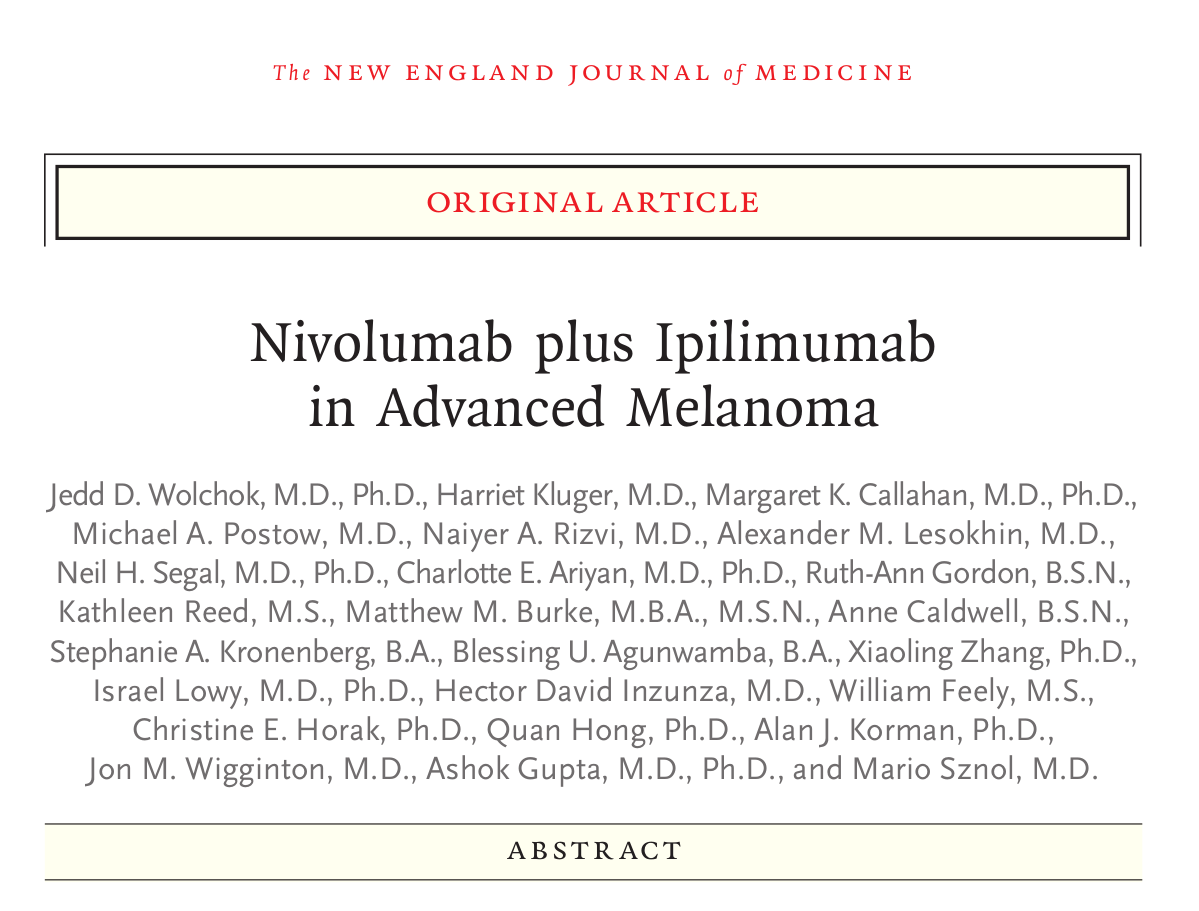
\includegraphics[scale=0.25]{wolchok.png}
\end{frame}

\begin{frame}{Table of results: Response to therapy}
\begin{itemize}
	\item Advanced melanoma is an aggressive form of skin cancer that until recently was almost uniformly fatal. 
	\item In rare instances, a patient's melanoma stopped progressing or disappeared altogether when the patient's immune system successfully mounted a response to the cancer. 
	\item Those observations led to research into therapies that might trigger an immune response in cancer. 
	\item Some of the	most notable successes have been in melanoma, particularly with two new therapies, nivolumab
	and ipilimumab. \pause 
	\item A 2013 report in the New England Journal of Medicine by Wolchok et al.a\footnote{\tiny \url{https://www.nejm.org/doi/full/10.1056/nejmoa1302369}} reported the results
	of a study in which patients were treated with both nivolumab and ipilimumab. 53 patients were given the new regimens concurrently, and the response to therapy could be evaluated in 52 of the 53.
\end{itemize}
\end{frame}

\begin{frame}{Phase 1 trial in patients with advanced melanoma\footnote{\tiny \url{https://www.nejm.org/doi/full/10.1056/nejmoa1302369}}}
	\centering
	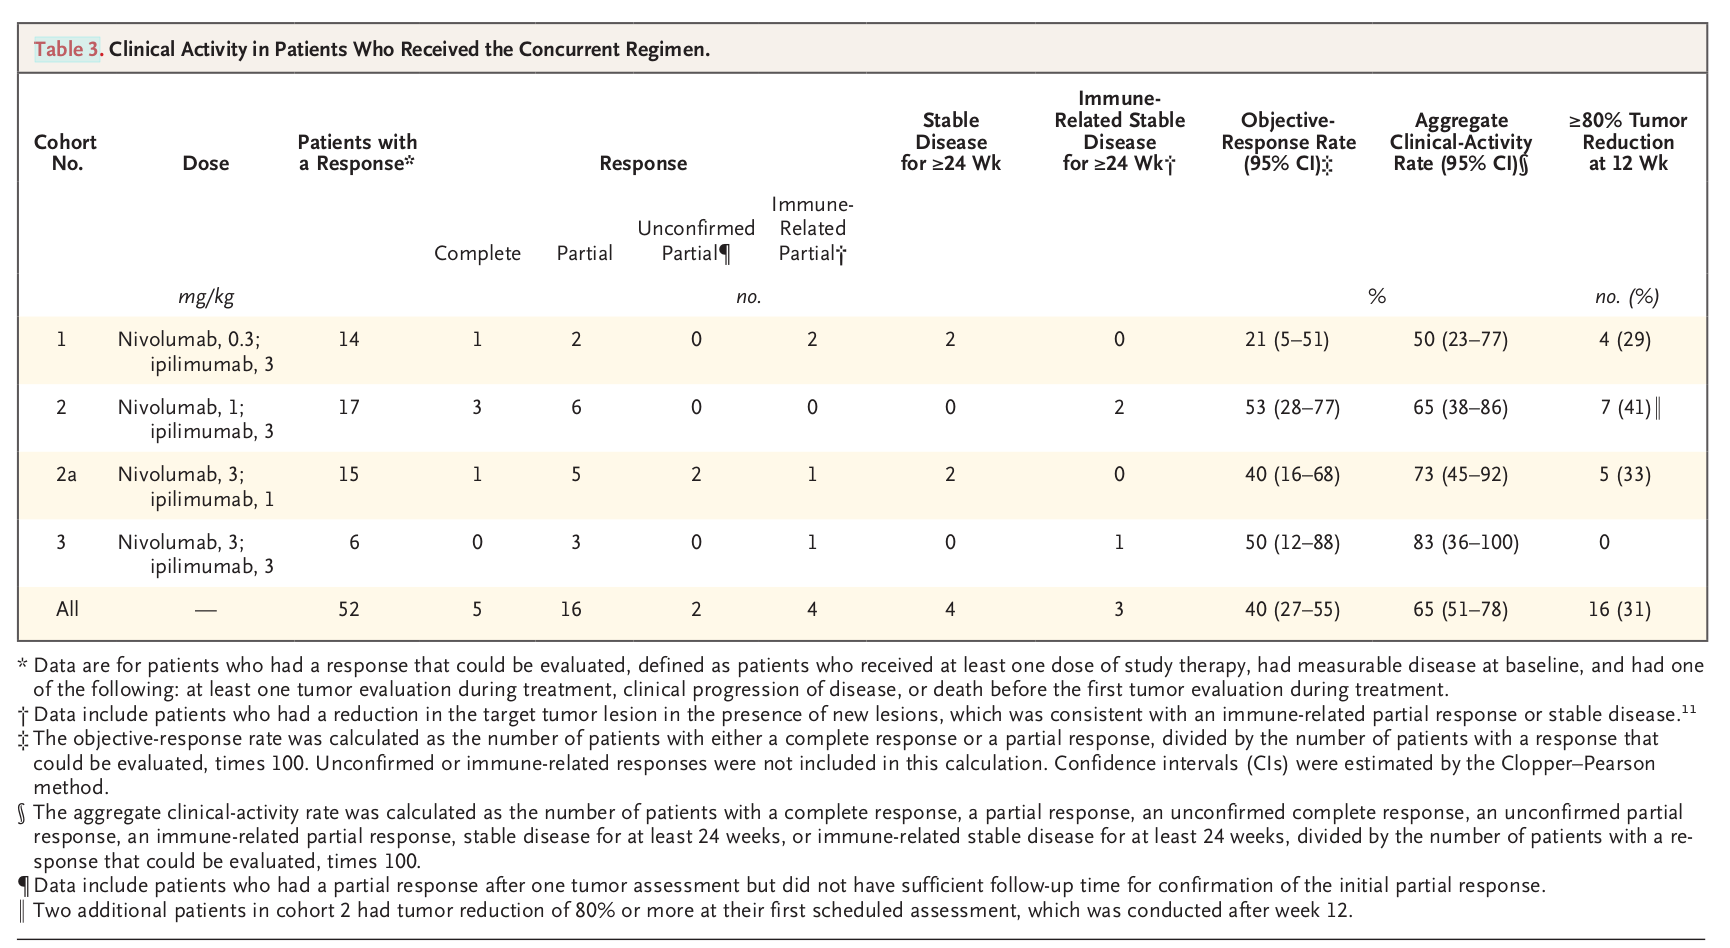
\includegraphics[scale=0.25]{wolchok2.png}
\end{frame}

\begin{frame}{How to interpret the 95\% CI of 40 [27-55] ?\footnote{\tiny this page is intentionally left blank}}
	
\end{frame}


\begin{frame}{Binomial Data}
\begin{itemize}
	\item The data from this study are binomial data. 
	\item Event defined as a response to therapy.
	\item Suppose the number of patients who respond in a study like this is represented by the random
	variable Y, where Y is binomial with parameters n (the number of trials, where each trial is rep-
	resented by a patient) and $\pi$ (the unknown population proportion of response). This is denoted by $$Y\sim Binom(n,\pi)$$
	\item In this section we are concerned about the inference of $\pi$
\end{itemize}
\end{frame}


%\section{Power and Sample Size}

\begin{frame}[fragile,plain]
\begin{knitrout}\tiny
\definecolor{shadecolor}{rgb}{0.969, 0.969, 0.969}\color{fgcolor}

{\centering 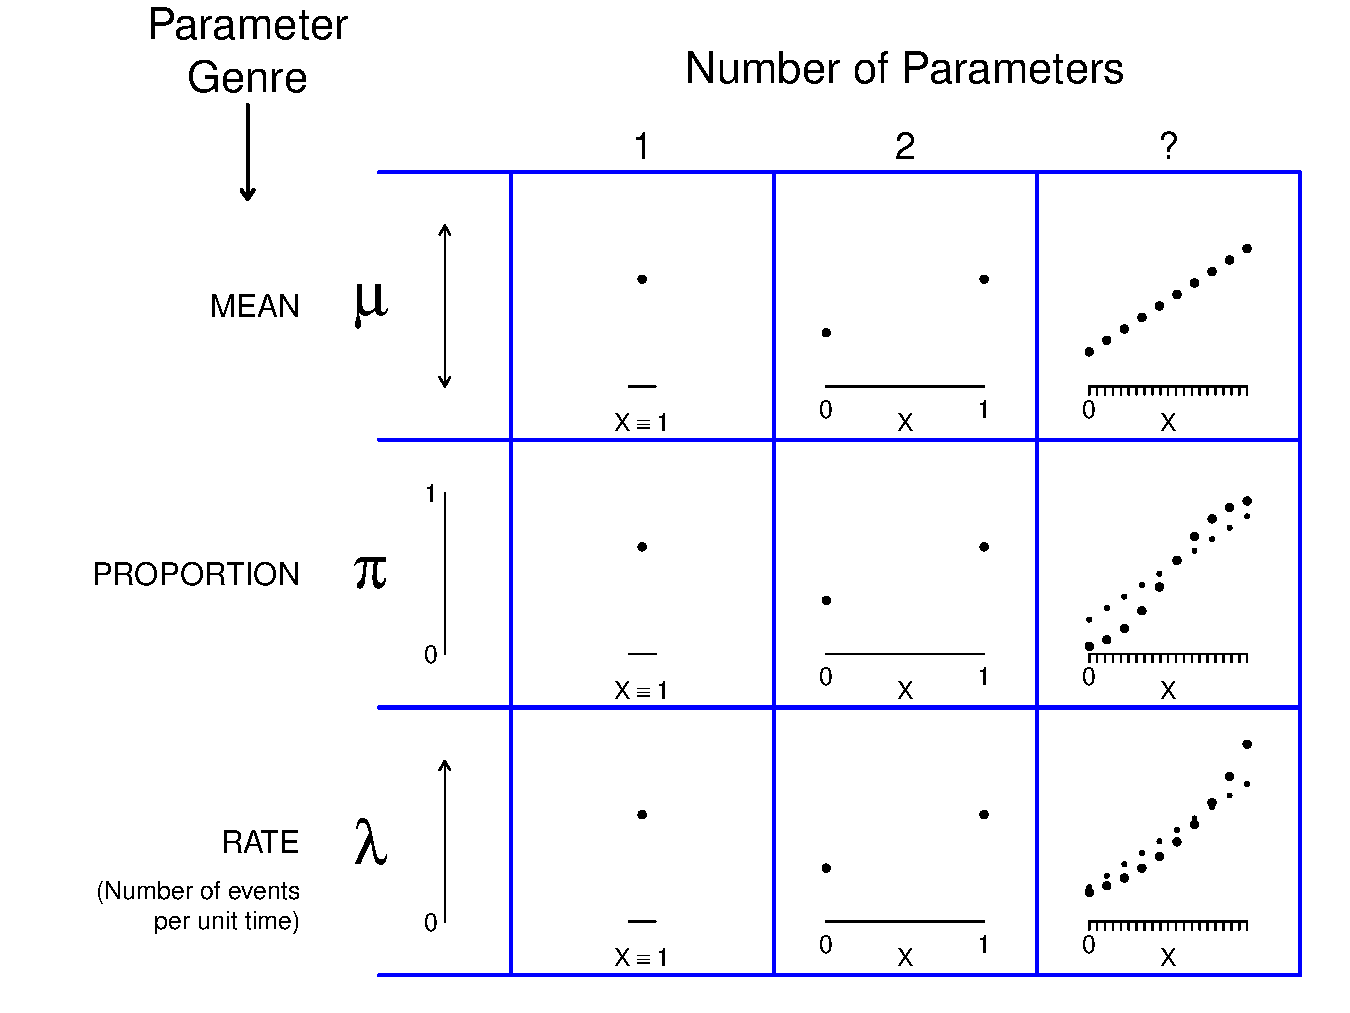
\includegraphics[width=\maxwidth]{figure/unnamed-chunk-1-1} 

}



\end{knitrout}
\end{frame}


\section{Binomial Model for Sampling Variability of Proportion/Count in a Sample}




\begin{frame}
	\frametitle{The Binomial Distribution: what it is}
	\small
	\begin{itemize}
		\setlength\itemsep{0.5em}
		\item It is the $n+1$ probabilities $p_{0}, p_{1}, ..., p_{y}, ..., p_{n}$ of observing 
		$0, 1, 2, \dots , n$ ``events''  in \underline{$n$ independent realizations of a Bernoulli random variable} $Y$:
		$$
		Y = \begin{cases}
		1 & P(Y=1) = \pi \\
		0 & P(Y=0) = 1-\pi
		\end{cases}	
		$$
		The number is the sum of $n$ i.i.d. Bernoulli random variables.	(\emph{such as in SRS of $n$ individuals}) \pause 
		\item Each of the $n$ observed elements is binary (0 or 1) %\pause 
		\item There are $2^{n}$ possible \textit{sequences} ... but only $n+1$ possible \textit{values}, 
		i.e. $0/n,\;1/n,\;\dots ,\;n/n$  \emph{(can think of $y$ as sum of $n$ Bernoulli random variables)} 
		\item Note: it is better to work in same scale as the parameter, i.e., in [0,1]. Not the [0,n] count scale.
	\end{itemize}
\end{frame}	

\begin{frame}
	\frametitle{The Binomial Distribution: what it is}
	\begin{itemize}
		\setlength\itemsep{0.5em}
		\item Apart from  ($n$), the probabilities $p_{0}$ to $p_{n}$ depend on only 1 parameter:
		\begin{itemize}
			\item the probability that a selected individual will be ``positive''  i.e.,
			\item the proportion of ``positive'' individuals in sampled population
		\end{itemize}
		
		\item Usually denote this (un-knowable) proportion by $\pi$
		
		\begin{tabular}{lcc}
			\hline
			Author & \textbf{Parameter} & \textbf{Statistic} \\
			\hline
			Clayton \& Hills   & $\pi $ & $p= D/N$ \\
			Hanley et al. & $\pi $ & $p= y/n$ \\
			DVB & p &$\hat{p} = y/n$ \\
			M\&M, Baldi \& Moore & p &$\hat{p} = y/n$ \\
			Miettinen& P & $p=y/n$ \\
			\hline
		\end{tabular}
		\item
		Shorthand:  $Y\sim\; \textrm{Binomial}(n, \pi)$.
	\end{itemize}
\end{frame}


\begin{frame}{Example: Searching for LeBron (DVB Chapter 17)}
	\begin{columns}
		\begin{column}{0.2\textwidth}
			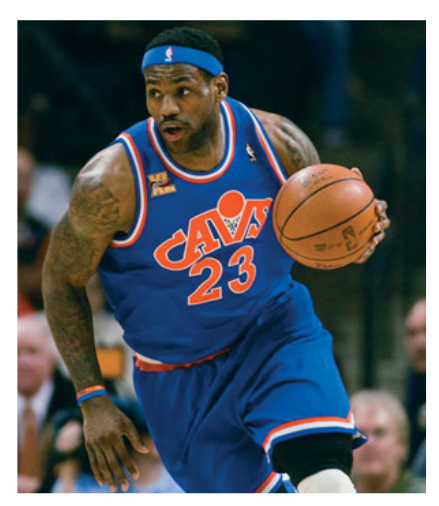
\includegraphics[scale=0.2]{lebron.png}
		\end{column}
		\begin{column}{0.78\textwidth}
			\small
			\begin{itemize}
				\item Assume LeBron cards are distributed at random and
				that 20\% of the cards in cereal boxes are LeBron $\to$ P(LeBron)= 0.20
				\item We'll call the act of opening each box a trial
				\item Let $Y$ be the number of LeBron cards you get among $n$ cereal boxes
				\item Is $Y\sim Binomial(n,0.2)$? \pause
				\begin{enumerate}
					\item Only two possible outcomes on each trial. Either you get LeBron's picture (event), or you don't (no event).
					\item The probability of success is the same on every trial. (10\% Condition in DVB)
					\item The trials are independent. Finding LeBron in the first box does not change what might happen when you reach for the next box
				\end{enumerate}
			\end{itemize}
		\end{column}
	\end{columns}
	
\end{frame}


\begin{frame}{A note on the Independence (10\% Condition)}
	\small 
	\begin{itemize}
		\item One of the important requirements for Bernoulli trials is that the trials be independent. 
		\item Reasonable assumption when tossing a coin or rolling a die.
		\item Becomes a problem when we're looking at situations involving samples chosen without replacement. 
		\item Technically, if exactly 20\% of the boxes have LeBron James cards, then when you find one, you’ve reduced the number of remaining LeBron James cards. 
		%\item With a few million boxes of cereal, though, the difference is hardly worth mentioning.
		\item If you knew there were 2 LeBron James cards hiding in the 10 boxes on the market shelf, then finding one in the first box you try would
		clearly change your chances of finding LeBron in the next box.
		\item If we had an infinite number of boxes, there wouldn't be a problem. It's
		selecting from a finite population that causes the probabilities to change, making
		the trials not independent. 
		\item If we look at less than 10\% of the population, we can pretend that the
		trials are independent and still calculate probabilities that are quite accurate.
	\end{itemize}
\end{frame}

\begin{comment}
\frame{\frametitle{Example} 

\begin{itemize}
\setlength\itemsep{1em}
\item Suppose a woman plans to have 3 children. 
\item Suppose at each birth, 
$$P(\textrm{female child}) = 1/2$$ and the sex of the child at each birth is
independent of the sex at any previous birth. 
\item What is the probability of having all daughters?
\end{itemize} 

}

\frame{\frametitle{The binomial distribution}

\vspace*{-0.5in}

\begin{figure}
\begin{center}
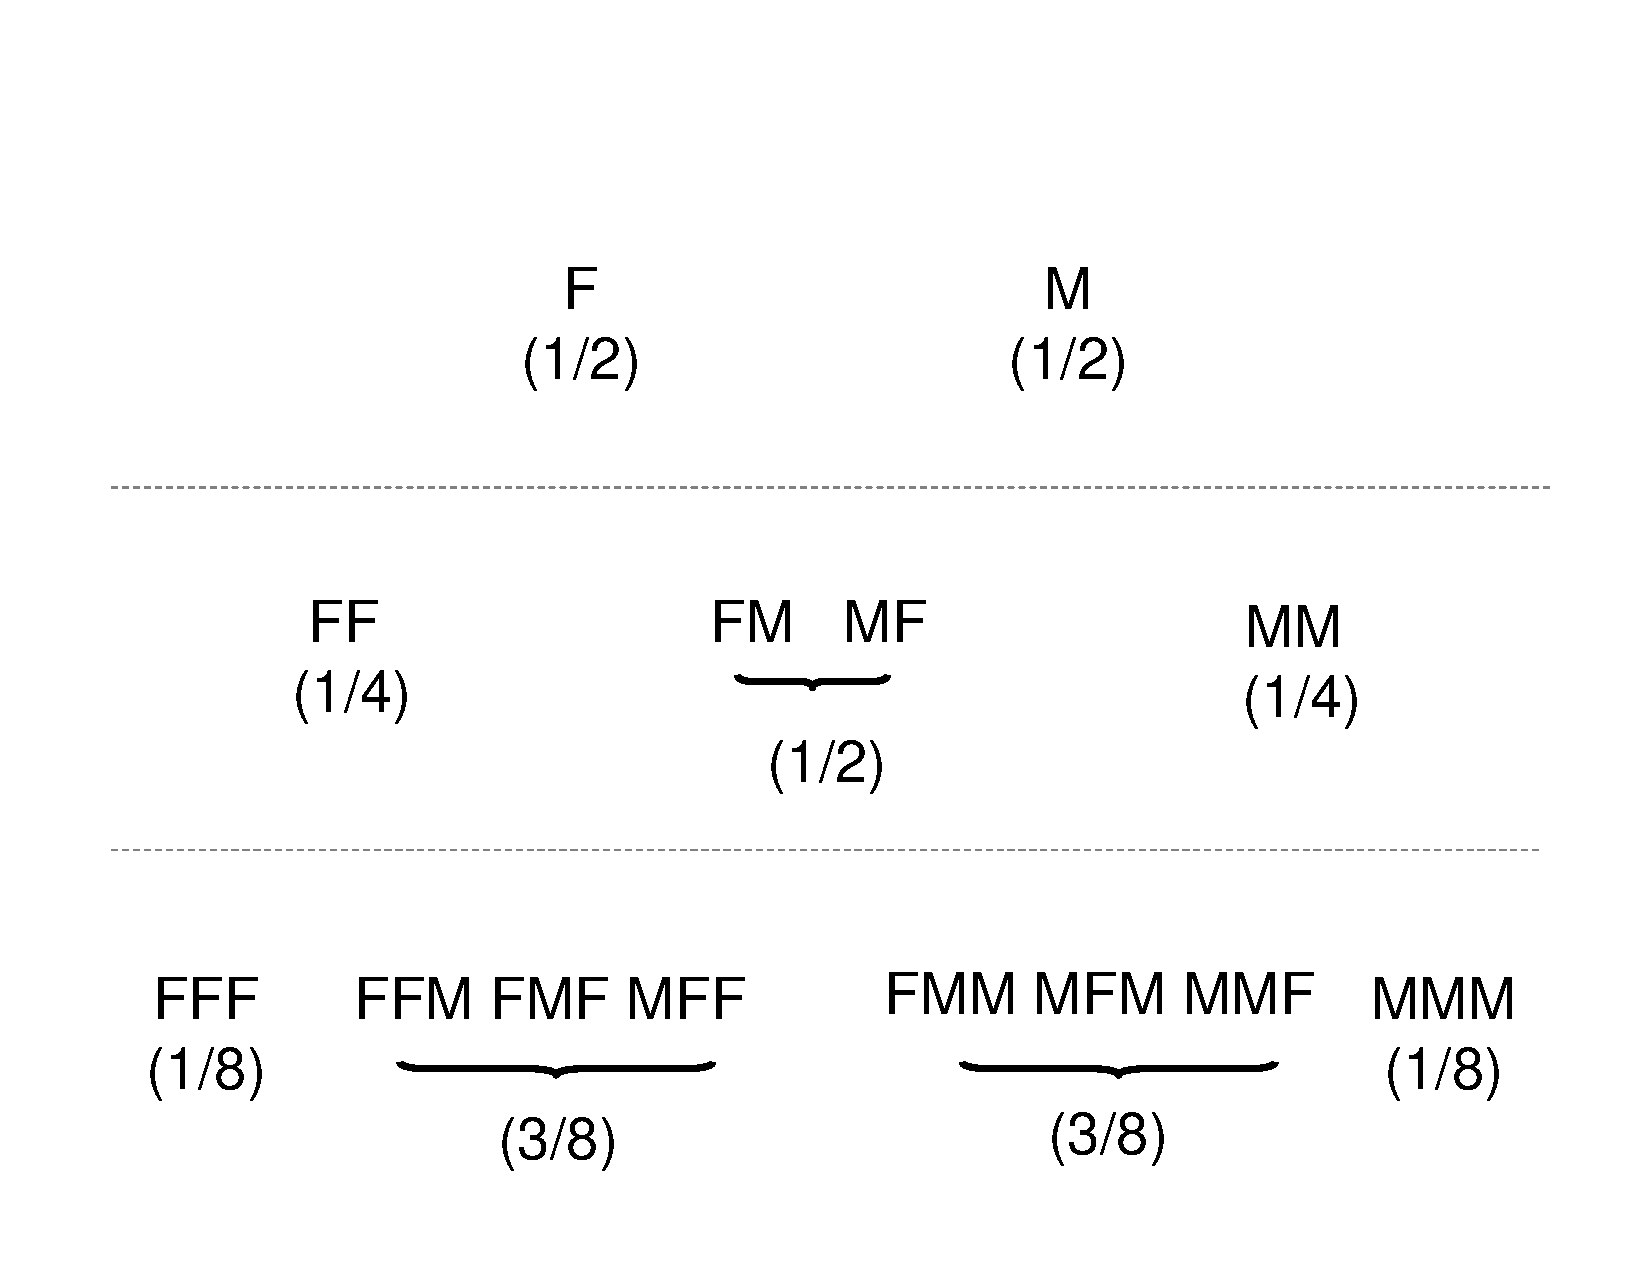
\includegraphics[scale=0.4,angle=0]{binomial.pdf}
\end{center}
\end{figure}
}
\end{comment}


\frame{\frametitle{The binomial distribution} 
	
	\begin{itemize}
		\item $Y$: the total number of LeBron cards you find in $n$ boxes
		\item $n$: the number of cereal boxes you will open
		\item $\pi$: the probability of getting LeBron card in any box
	\end{itemize}
	
	Then: \\ \ \\
	\[ P(Y=k) =
	\frac{n!}{(n-k)!k!}\pi^k(1-\pi)^{(n-k)}\] \ \\ \ \\ where $n! =
	1\times2\times3\times ... \times (n-1)\times n$, and $0!=1$. \\ \ \\
	
	$$
	\frac{n!}{(n-k)!k!} \equiv \binom{n}{k} \equiv \textcolor{white}{te}_nC_k 
	$$
	
}

\begin{frame}[fragile]{}
\begin{knitrout}\tiny
\definecolor{shadecolor}{rgb}{0.969, 0.969, 0.969}\color{fgcolor}

{\centering 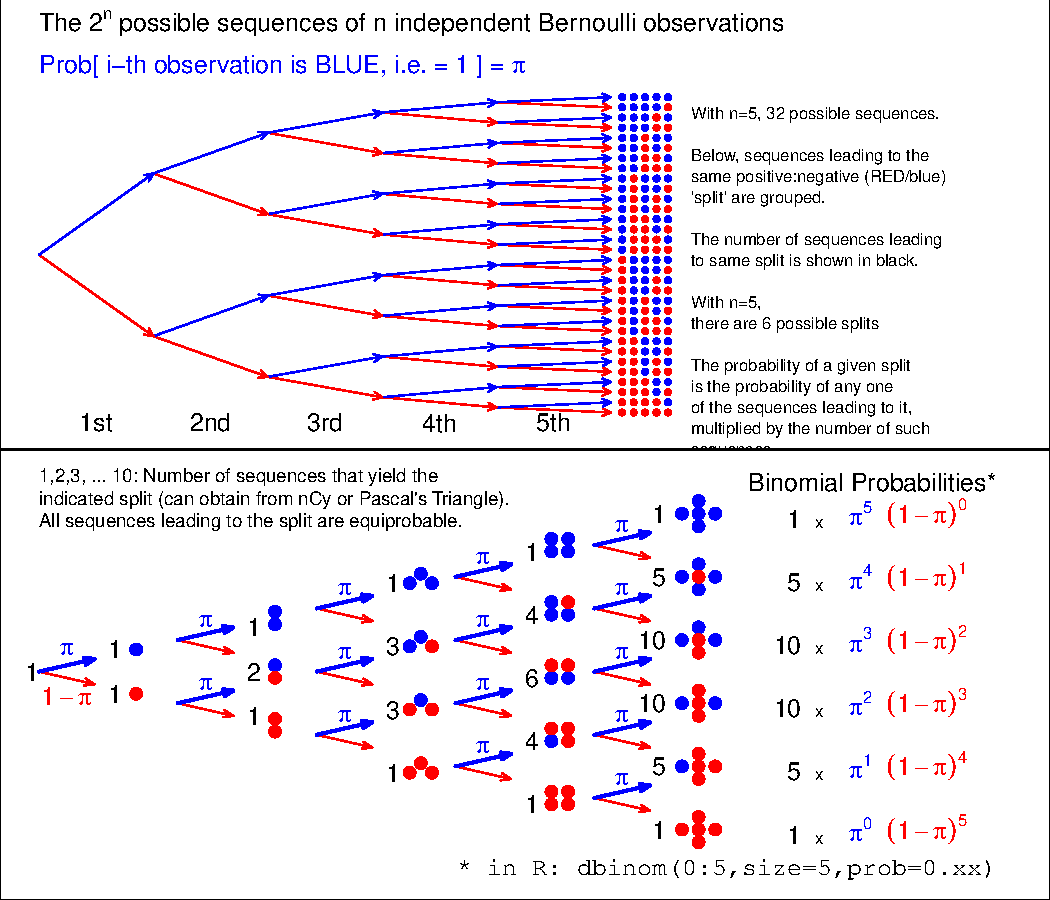
\includegraphics[width=\maxwidth]{figure/unnamed-chunk-2-1} 

}



\end{knitrout}
\end{frame}


\begin{frame}[fragile]{Calculating binomial probabilities in R}
	
	The probability of getting 3 LeBron cards in 10 boxes:
	
	\vspace{.21in}
	
	$P(Y=3) = \frac{10!}{7!3!}0.2^3(1-0.2)^{7}$ \\ \ \\
	which can be solved in R using:
\begin{knitrout}\tiny
\definecolor{shadecolor}{rgb}{0.969, 0.969, 0.969}\color{fgcolor}\begin{kframe}
\begin{alltt}
\hlstd{stats}\hlopt{::}\hlkwd{dbinom}\hlstd{(}\hlkwc{x} \hlstd{=} \hlnum{3}\hlstd{,} \hlkwc{size} \hlstd{=} \hlnum{10}\hlstd{,} \hlkwc{prob} \hlstd{=} \hlnum{0.2}\hlstd{)}
\end{alltt}
\begin{verbatim}
## [1] 0.2
\end{verbatim}
\end{kframe}
\end{knitrout}
\end{frame}

\begin{frame}[fragile]{The probability mass function (pmf)}
	
\begin{knitrout}\tiny
\definecolor{shadecolor}{rgb}{0.969, 0.969, 0.969}\color{fgcolor}\begin{kframe}
\begin{alltt}
\hlkwd{plot}\hlstd{(}\hlnum{0}\hlopt{:}\hlnum{10}\hlopt{/}\hlnum{10}\hlstd{,} \hlkwd{dbinom}\hlstd{(}\hlkwc{x} \hlstd{=} \hlnum{0}\hlopt{:}\hlnum{10}\hlstd{,} \hlkwc{size} \hlstd{=} \hlnum{10}\hlstd{,} \hlkwc{prob} \hlstd{=} \hlnum{0.2}\hlstd{),} \hlkwc{type} \hlstd{=} \hlstr{"h"}\hlstd{)}
\end{alltt}
\end{kframe}

{\centering 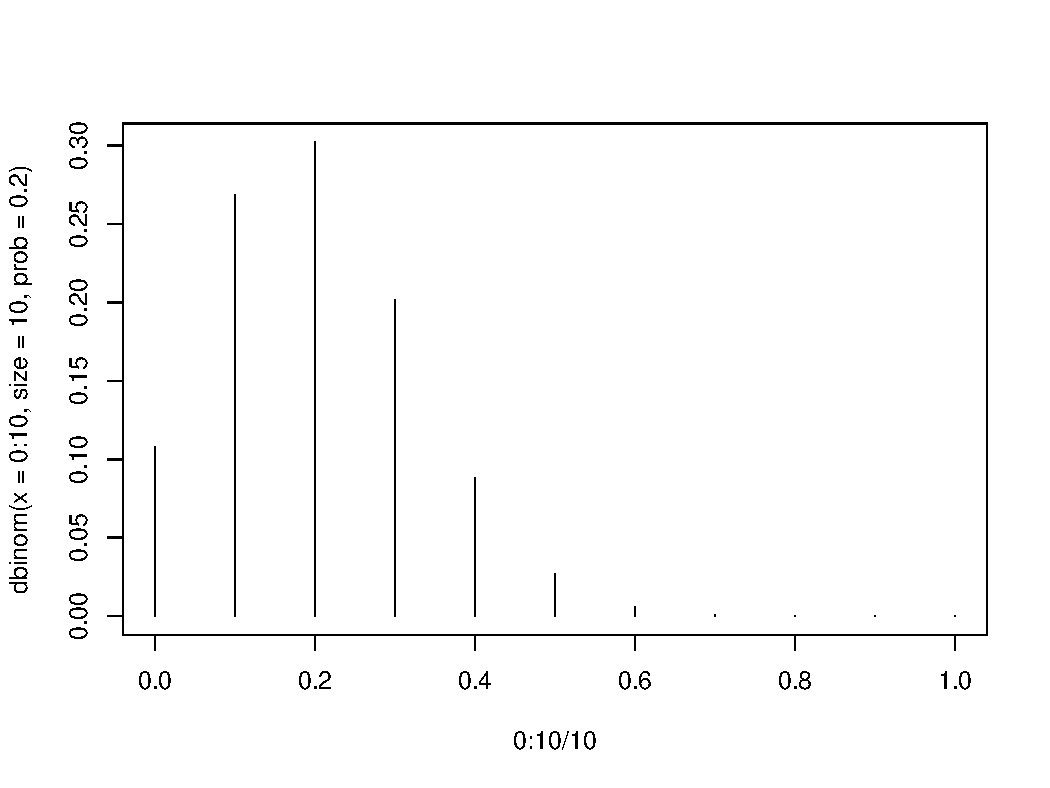
\includegraphics[width=\maxwidth]{figure/unnamed-chunk-4-1} 

}



\end{knitrout}
\end{frame}

\begin{frame}[fragile]{What do we use it for?}
	\small
	\begin{itemize}
		\setlength\itemsep{0.7em}
		\item to make inferences about $\pi$ from  observed  proportion $p= y/n.$ \pause 
		\item to make inferences in more complex situations, e.g. 
		\begin{itemize}
			\setlength\itemsep{0.4em}
			\item Prevalence Difference: $\pi _{1} - \pi _{0}$
			\item Risk Difference (RD): $\pi _{1} - \pi _{0}$
			\item Risk Ratio, or its synonym Relative Risk (RR): $\pi _{1}\:/\:\pi _{0}$
			\item Odds Ratio (OR): $[\: \pi _{1}/(1-\pi _{1})\:] \: / \: [\: \pi _{0}\: / \: (1-\pi _{0}) \: ]$
			\item Trend in several $\pi $'s
		\end{itemize}
	\end{itemize}
\end{frame}


\frame{\frametitle{Requirements for $y$ to have a Binomial (n, $\pi $) distribution} 
	\begin{enumerate}
		\item Fixed sample size $n.$ 
		\item Elements selected at random (i.e. same probability of being sampled) and independent of each other $\to$ 10\% condition in DVB (LeBron James example).
		\item Each element in ``population'' is 0 or 1, but we are only interested in estimating proportion  ($\pi $) of 1's;  we are not interested in individuals. 
		\item Denote by $y_{i}$ the value of the $i$-th sampled element.  P($y_{i}=1)$ is constant (it is $\pi$) across $i$.
\end{enumerate} }

\begin{comment}
\begin{frame}
\begin{figure}
\begin{center}
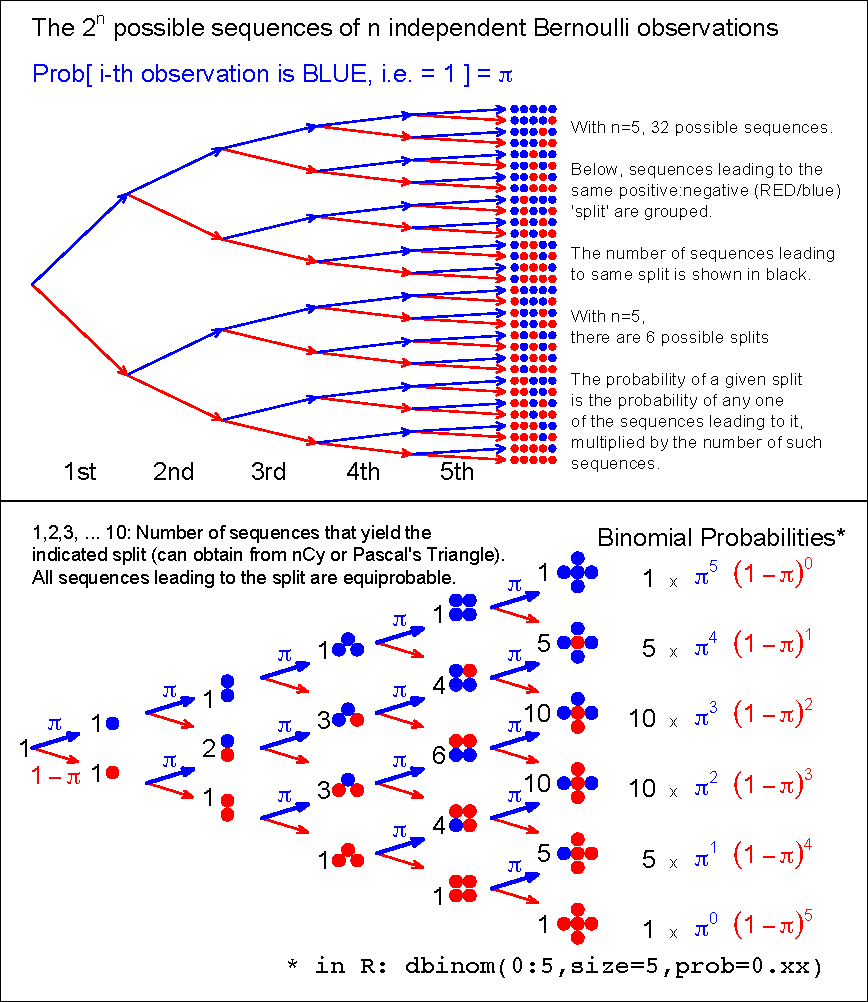
\includegraphics[scale=0.55]{BinomialTree2018.pdf}
\caption{\scriptsize From 5 (independent and identically distributed) Bernoulli observations to Binomial $(n=5), \: \pi \textrm{ unspecified}$.}
%There are $2^n$ possible (distinct) sequences of 0's and 1's, each with its probability. We are not interested in these $2^n$ probabilities, but in the probability that the sample  contains $y$ 1's and $(n-y)$ 0's. There are only ($n$+1) possibilities for $y$, namely 0 to $n.$ Fortunately, each of the $nC_y$ sequences that lead to the same sum or count ($y$), has the same probability. So we group the 2$^n$ sequences into $(n+1)$ sets, according to the sum or count. Each sequence in the set with  $y$ 1's and $(n-y)$ 0's has the same probability, namely $\pi ^{y}(1-\pi )^{n-y}$. Thus, in lieu of adding all such probabilities, we simply multiply this  probability by the number, $^{n}C _{y}$ -- shown in black -- of unique sequences in the set. Check: the numbers in black add to 2$^n.$ Nowadays, the $(n+1)$ probabilities are easily obtained by supplying a value for the \texttt{prob} argument in the \texttt{R} function \texttt{dbinom}, instead of  computing the binomial coefficient $nC_y$ by hand.}
\end{center}
\end{figure}
\end{frame}
\end{comment}




\begin{comment}
\begin{frame}{Does the Binomial Distribution Apply if... ?}

\small
\begin{tabular}{lrl}
\hline
Interested in & $\pi$      &  the proportion of 16 year old girls  \\
&              &   in Qu\'{e}bec protected against rubella \\
& & \\
Choose        & $n=100$ & girls: 20 at random from each of 5 randomly \\
&                &selected schools [`cluster' sample] \\
& & \\
Count & $y$ & how many of the $n=100$  are protected \\
& & \\

\multicolumn{3}{l}{$\bullet$ Is $y \sim \textrm{Binomial}(n = 100, \pi $)? } \\
\hline
& & \\
``SMAC'' & $\pi$      &   P(abnormal$\:|\:$Healthy) =0.03 for each chemistry \\
& &                       in Auto-analyzer with $n=18$ channels  \\
&         &  \\
Count            & y$ $&  How many of $n=18$  give abnormal result.  \\
& & \\
\multicolumn{3}{l}{$\bullet$ Is $y \sim \textrm{Binomial}(n = 18, \pi =0.03$)? (cf. Ingelfinger: Clin. Biostatistics) } 
\end{tabular}
\end{frame}


\begin{frame}{Does the Binomial Distribution Apply if... ?}

\small
\begin{tabular}{lrl}
\hline

Interested in & $\pi _{u}$      &   proportion in `usual' exercise classes and in  \\
& $\pi _{e}$      &   expt'l. exercise classes who `stay the course'  \\
& & \\
Randomly & 4   & classes of\\ 
Allocate    &  \underline{25} & students each to usual course \\
& $n_{u} = 100$ &  \\
& 4  & classes of\\
&  \underline{25} & students each to experimental course \\
& $n_{e} =100$ &  \\

Count & $y_u$ & how many of the $n_{u}=100$ complete course \\
& $y_e$ & how many of the $n_{e}=100$  complete course \\

\multicolumn{3}{l}{$\bullet$ Is $y_{u} \sim \textrm{Binomial}(n_{u} = 100,  \pi _{u}$) ?
\ \  Is $y_{e} \sim \textrm{Binomial}(n_{e} = 100,  \pi _{e}$) ?} \\
& & \\
\hline
\end{tabular}
\end{frame}



\begin{frame}{Does the Binomial Distribution Apply if... ?}

\small
\begin{tabular}{lrl}
\hline
Sex Ratio & $n=4$& children in each family  \\
& $y$ & number of girls in family \\
& & \\
\multicolumn{3}{l}{$\bullet$ Is variation of y across families Binomial (n = 4, $\pi $ = 0.49)?} \\
\hline
Pilot  &   &To estimate proportion $\pi$ of population that\\ 
Study&   &  is eligible \& willing to participate in long-term\\
&   & research study, keep recruiting until obtain   \\
& $y=5$ &  who are. Have to approach $n$ to get $y$. \\
& & \\
\multicolumn{3}{l}{$\bullet$ Can we treat $y \sim \textrm{Binomial}(n, \pi$)?} \\
\hline
\end{tabular}
\end{frame}
\end{comment}

\begin{frame}{Calculating Binomial probabilities - Exactly}
	
	
	
	\begin{itemize}
		\item  probability mass function (pmf): $P(Y=k) =
		\frac{n!}{(n-k)!k!}p^k(1-p)^{(n-k)}$
		\item in \texttt{R}: \texttt{dbinom(), pbinom(), qbinom()}: \newline probability mass, distribution/cdf, and quantile functions.
	\end{itemize}
	
\end{frame}


\begin{frame}{Mean and Variance of Bernoulli Random Variable}
	\begin{itemize}
		\item To derive the formulas for the mean and standard deviation of a Binomial model we start with
		the most basic situation.
		\item Consider a single Bernoulli trial with probability of an event $\pi$. Let's find the mean and
		variance of the number of events ('successes').
	\end{itemize}
\vspace*{1.5in}
	
%	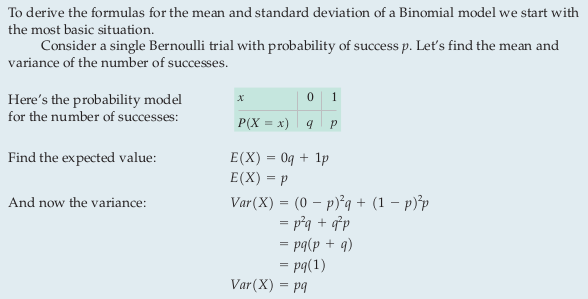
\includegraphics[scale=1,width=\linewidth]{binom_math1.png}
\end{frame}


\begin{frame}{Mean and Variance of Binomial Random Variable}
%	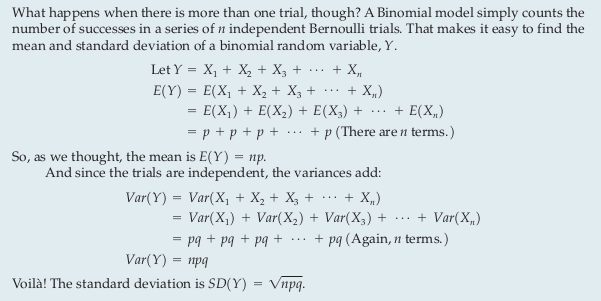
\includegraphics[scale=1,width=\linewidth]{binom_math2.png}
	\begin{itemize}
	\item What happens when there is more than one trial, though? A Binomial model simply counts the
	number of successes in a series of $n$ independent Bernoulli trials. That makes it easy to find the
	mean and standard deviation of a binomial random variable, $Y$.
\end{itemize}
\vspace*{1.5in}
\end{frame}


\begin{frame}{Calculating Binomial probabilities - Using an approximation}
	
	\small
	\begin{itemize}
		\item Poisson Distribution ($n$ large;  small $\pi$)
		\item Normal (Gaussian) Distribution ($n$ large or midrange $\pi $) \footnote{\footnotesize
			For when you don't have access to software or Tables, e.g, on a plane} 
		\begin{itemize}
			\item Have to specify \textit{scale}. Say $n=10$, whether summary is a 
			\begin{tabular}{rllcc}
				&  \textbf{r.v. }        &  \textbf{e.g.} & \textbf{E} & \textbf{SD} \\ 
				\hline
				count:          &  $y$        &  2 & $n \times \pi$ & $\sqrt{n \times \pi \times (1-\pi)}$ \\
				& & & & \\
				& & & & $\sqrt{n} \times \sigma_{Bernoulli}$ \\
				
				& & & & \\
				proportion:   & $p=y/n$  & 0.2 & $ \pi$ & $ \sqrt{\pi \times (1-\pi) / n}$ \\
				& & & & \\
				
				& & & &  $\sigma_{Bernoulli} / \sqrt{n}$\\
				
				& & & & \\
				percentage: &$100p\%$ & 20\% & $100 \times \pi$ & $100 \times SD[p]$ \\
				\hline
			\end{tabular}
			\item same core calculation for all 3 [only the \textit{scale} changes]. JH prefers (0,1), the same scale as $\pi.$
			
		\end{itemize}
		
	\end{itemize}
	
\end{frame}



\begin{frame}[fragile]{Normal approximation to binomial is the CLT in action}
\begin{knitrout}\tiny
\definecolor{shadecolor}{rgb}{0.969, 0.969, 0.969}\color{fgcolor}

{\centering 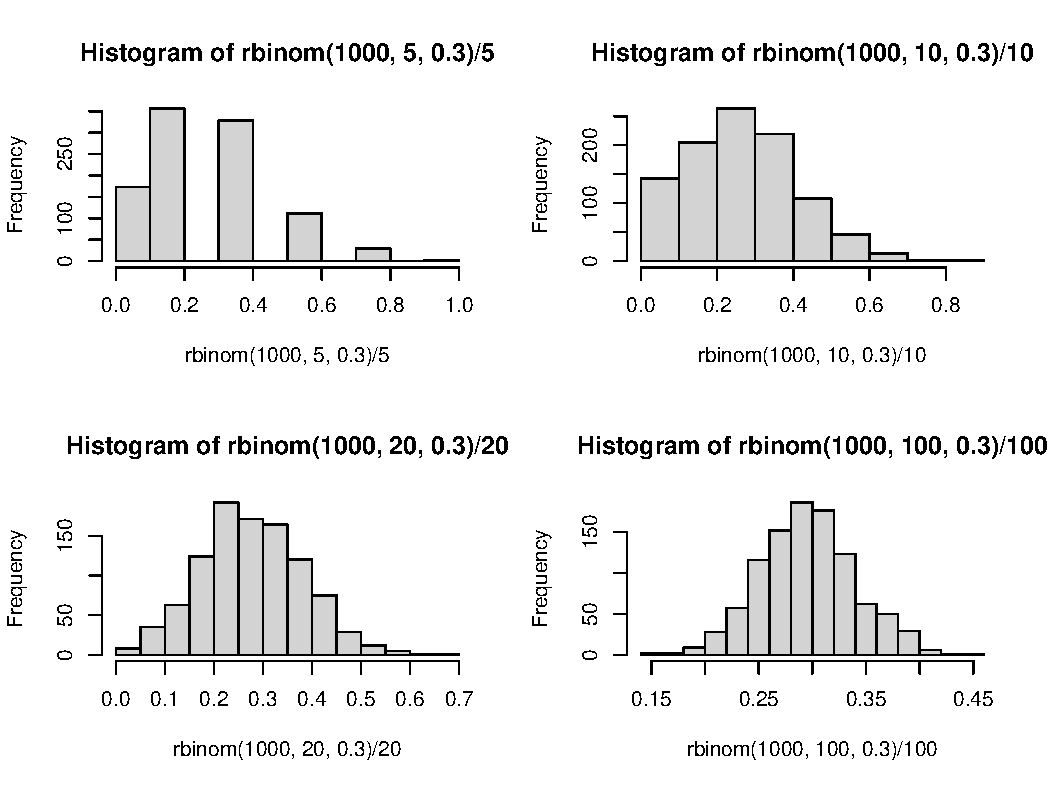
\includegraphics[width=\maxwidth]{figure/unnamed-chunk-5-1} 

}



\end{knitrout}
\end{frame}


\begin{frame}[fragile]{Normal approximation to binomial is the CLT in action}
\begin{knitrout}\tiny
\definecolor{shadecolor}{rgb}{0.969, 0.969, 0.969}\color{fgcolor}

{\centering 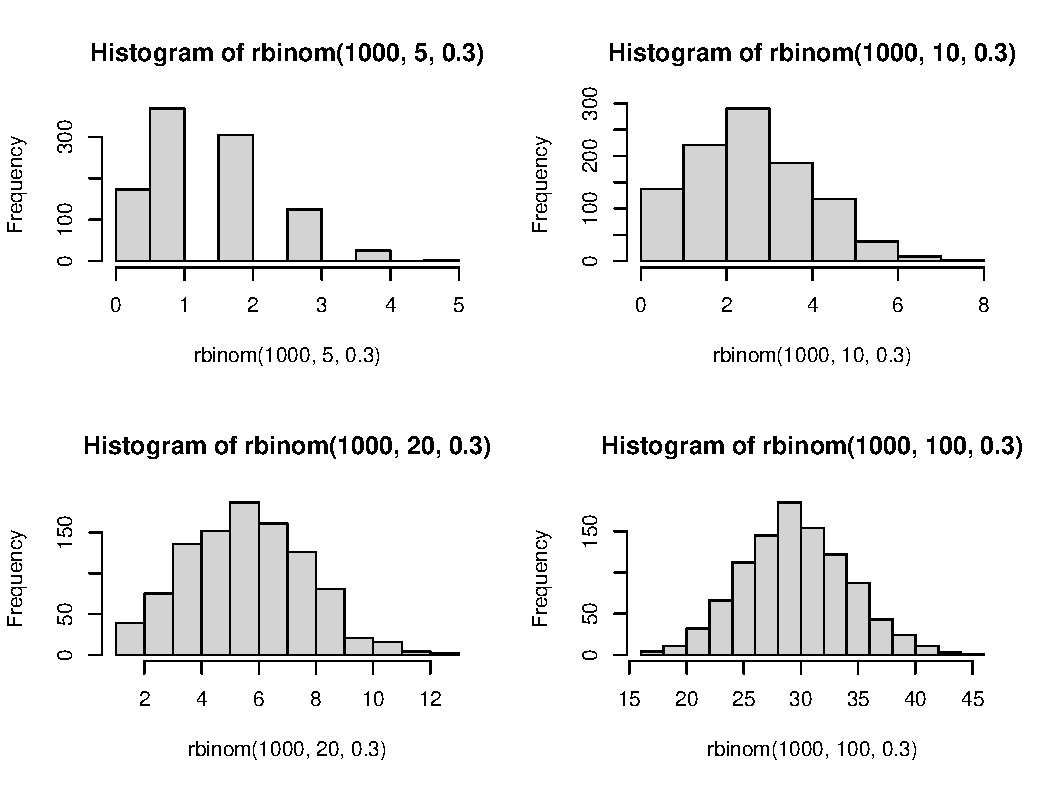
\includegraphics[width=\maxwidth]{figure/unnamed-chunk-6-1} 

}



\end{knitrout}
\end{frame}

\begin{frame}{Example 1 from AAO Unit 21}
	A drug manufacturer claims that its flu vaccine is 85\% effective; in other words, each person who is vaccinated stands an 85\% chance of developing immunity. Suppose that 200 randomly selected people are vaccinated. Let $Y$ be the number that develops immunity.
	
	\begin{enumerate}
		\item What is the distribution of $Y$?
		\item What is the mean and standard deviation for $Y$?
		\item What is the probability that between 165 and 180 of the 200 people who were vaccinated
		develop immunity? (Hint: Use a normal distribution to approximate the distribution of $Y$)
	\end{enumerate}
\end{frame}


\begin{frame}[fragile]{Example 1 from AAO Unit 21 - Exact Method}
	
\begin{knitrout}\tiny
\definecolor{shadecolor}{rgb}{0.969, 0.969, 0.969}\color{fgcolor}\begin{kframe}
\begin{alltt}
\hlstd{mosaic}\hlopt{::}\hlkwd{xpbinom}\hlstd{(}\hlkwc{q} \hlstd{=} \hlkwd{c}\hlstd{(}\hlnum{165}\hlstd{,} \hlnum{180}\hlstd{),} \hlkwc{size} \hlstd{=} \hlnum{200}\hlstd{,} \hlkwc{prob} \hlstd{=} \hlnum{0.85}\hlstd{)}
\end{alltt}
\end{kframe}

{\centering 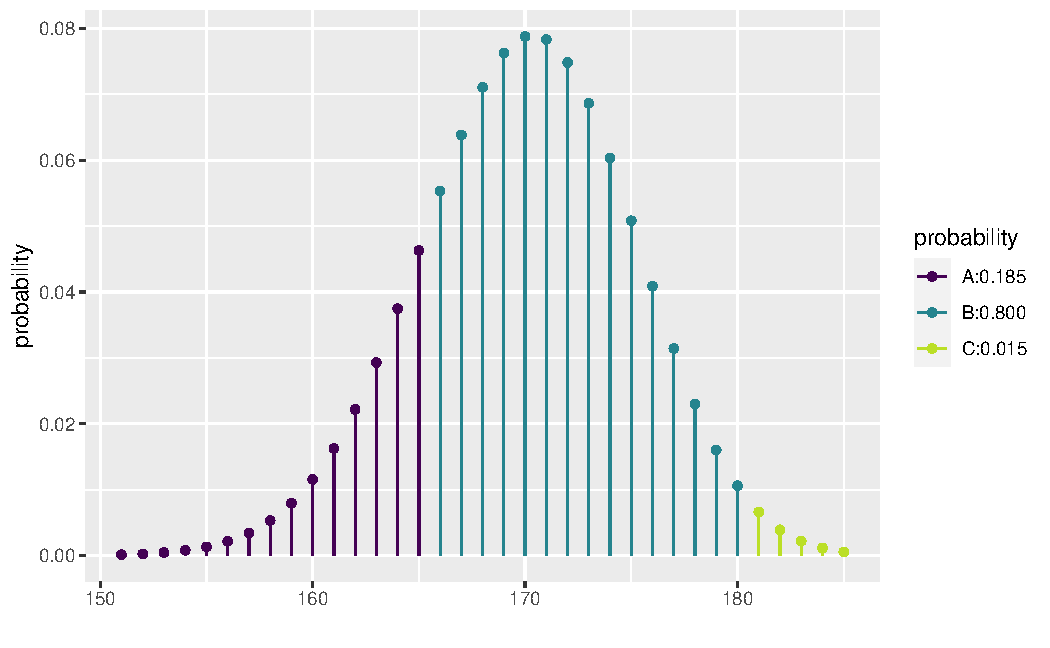
\includegraphics[width=\maxwidth]{figure/unnamed-chunk-7-1} 

}


\begin{kframe}\begin{verbatim}
## [1] 0.19 0.99
\end{verbatim}
\end{kframe}
\end{knitrout}
\end{frame}

\begin{frame}[fragile]{Example from AAO Unit 21- Normal Approximation}
	
\begin{knitrout}\tiny
\definecolor{shadecolor}{rgb}{0.969, 0.969, 0.969}\color{fgcolor}\begin{kframe}
\begin{alltt}
\hlstd{mosaic}\hlopt{::}\hlkwd{xpnorm}\hlstd{(}\hlkwc{q} \hlstd{=} \hlkwd{c}\hlstd{(}\hlnum{165}\hlstd{,}\hlnum{180}\hlstd{),} \hlkwc{mean} \hlstd{=} \hlnum{200} \hlopt{*} \hlnum{0.85}\hlstd{,}
\hlkwc{sd} \hlstd{=} \hlkwd{sqrt}\hlstd{(}\hlnum{200}\hlopt{*}\hlnum{0.85}\hlopt{*}\hlnum{0.15}\hlstd{))}
\end{alltt}
\end{kframe}

{\centering 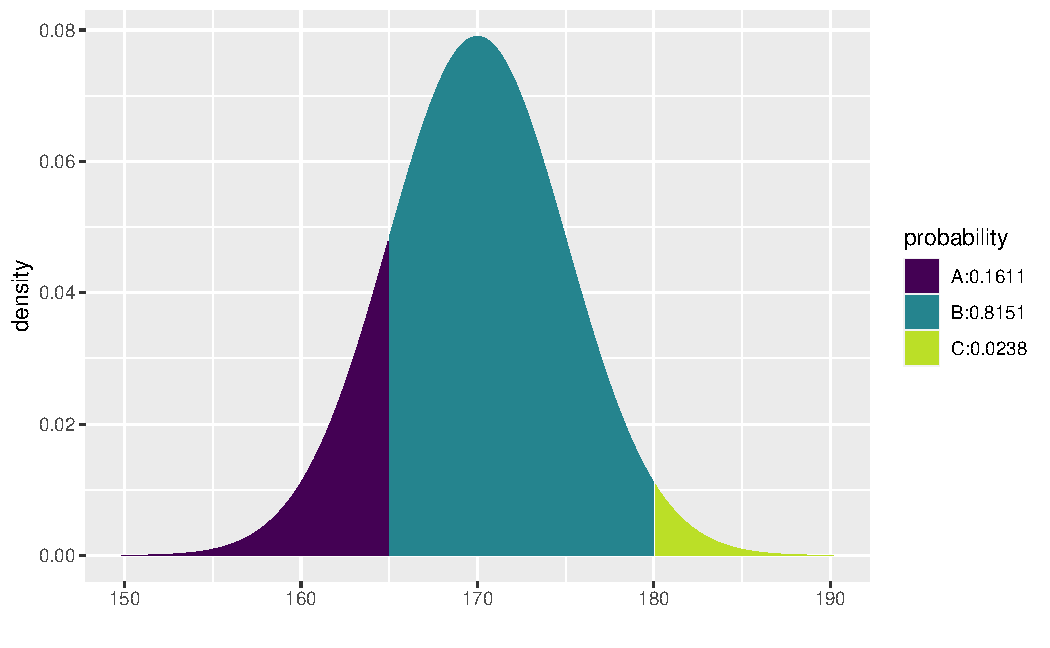
\includegraphics[width=\maxwidth]{figure/unnamed-chunk-8-1} 

}


\begin{kframe}\begin{verbatim}
## [1] 0.16 0.98
\end{verbatim}
\end{kframe}
\end{knitrout}
\end{frame}



\begin{frame}{Example 2 from AAO Unit 21}
	People with O- blood are called universal donors because most people can receive an O-blood transfusion. The probability of having blood type O- is 0.066. Suppose a random sample of five people show up during a blood drive to donate blood. Let $Y$ be the number of people with blood type O-.
	
	\begin{enumerate}
		\item What is the probability that none of the five people has blood type O-?
		\item What is the probability that exactly one of the five has blood type O-?
		\item What is the probability that no more than one of the five people has blood type O-?
		\item What is the probability that at least one of the five has blood type O-?
	\end{enumerate}
\end{frame}


\begin{frame}[fragile]{1. What is the probability that none of the five people has blood type O-?}
	
	$$ 
	P(Y = 0) = \binom{5}{0} 0.066^0 (1- 0.066)^5
	$$
	
	
\begin{knitrout}\tiny
\definecolor{shadecolor}{rgb}{0.969, 0.969, 0.969}\color{fgcolor}\begin{kframe}
\begin{alltt}
\hlstd{stats}\hlopt{::}\hlkwd{dbinom}\hlstd{(}\hlkwc{x} \hlstd{=} \hlnum{0}\hlstd{,} \hlkwc{size} \hlstd{=} \hlnum{5}\hlstd{,} \hlkwc{prob} \hlstd{=} \hlnum{0.066}\hlstd{)}
\end{alltt}
\begin{verbatim}
## [1] 0.71
\end{verbatim}
\begin{alltt}
\hlstd{(}\hlnum{1}\hlopt{-}\hlnum{0.066}\hlstd{)}\hlopt{^}\hlnum{5}
\end{alltt}
\begin{verbatim}
## [1] 0.71
\end{verbatim}
\end{kframe}
\end{knitrout}
	
\end{frame}



\begin{frame}[fragile]{2. What is the probability that exactly one of the five has blood type O-?}
	
	$$ 
	P(Y = 1) = \binom{5}{1} 0.066^1 (1- 0.066)^4
	$$
	
	
\begin{knitrout}\tiny
\definecolor{shadecolor}{rgb}{0.969, 0.969, 0.969}\color{fgcolor}\begin{kframe}
\begin{alltt}
\hlstd{stats}\hlopt{::}\hlkwd{dbinom}\hlstd{(}\hlkwc{x} \hlstd{=} \hlnum{1}\hlstd{,} \hlkwc{size} \hlstd{=} \hlnum{5}\hlstd{,} \hlkwc{prob} \hlstd{=} \hlnum{0.066}\hlstd{)}
\end{alltt}
\begin{verbatim}
## [1] 0.25
\end{verbatim}
\end{kframe}
\end{knitrout}
	
\end{frame}



\begin{frame}[fragile]{3. What is the probability that no more than one of the five people has blood type O-?}
	\footnotesize
	\begin{align*}
	P(Y \leq 1) & = P(Y = 0) + P(Y = 1) \\
	& = \binom{5}{0} 0.066^0 (1- 0.066)^5 + \binom{5}{1} 0.066^1 (1- 0.066)^4
	\end{align*}
	
	
\begin{knitrout}\tiny
\definecolor{shadecolor}{rgb}{0.969, 0.969, 0.969}\color{fgcolor}\begin{kframe}
\begin{alltt}
\hlstd{stats}\hlopt{::}\hlkwd{dbinom}\hlstd{(}\hlkwc{x} \hlstd{=} \hlnum{0}\hlstd{,} \hlkwc{size} \hlstd{=} \hlnum{5}\hlstd{,} \hlkwc{prob} \hlstd{=} \hlnum{0.066}\hlstd{)} \hlopt{+}
\hlstd{stats}\hlopt{::}\hlkwd{dbinom}\hlstd{(}\hlkwc{x} \hlstd{=} \hlnum{1}\hlstd{,} \hlkwc{size} \hlstd{=} \hlnum{5}\hlstd{,} \hlkwc{prob} \hlstd{=} \hlnum{0.066}\hlstd{)}
\end{alltt}
\begin{verbatim}
## [1] 0.96
\end{verbatim}
\begin{alltt}
\hlstd{stats}\hlopt{::}\hlkwd{pbinom}\hlstd{(}\hlkwc{q} \hlstd{=} \hlnum{1}\hlstd{,} \hlkwc{size} \hlstd{=} \hlnum{5}\hlstd{,} \hlkwc{prob} \hlstd{=} \hlnum{0.066}\hlstd{)}
\end{alltt}
\begin{verbatim}
## [1] 0.96
\end{verbatim}
\begin{alltt}
\hlstd{mosaic}\hlopt{::}\hlkwd{xpbinom}\hlstd{(}\hlkwc{q} \hlstd{=} \hlnum{1}\hlstd{,} \hlkwc{size} \hlstd{=} \hlnum{5}\hlstd{,} \hlkwc{prob} \hlstd{=} \hlnum{0.066}\hlstd{)}
\end{alltt}
\end{kframe}

{\centering 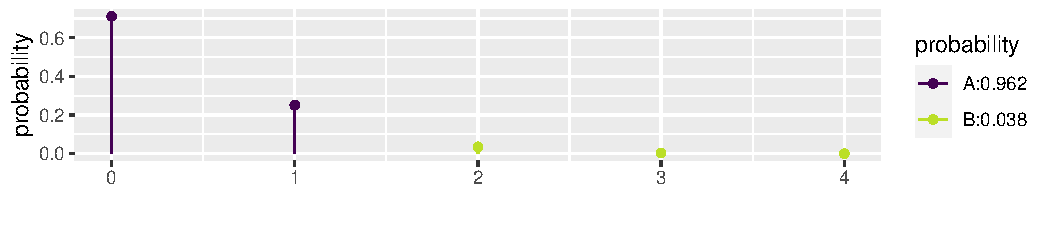
\includegraphics[width=\maxwidth]{figure/unnamed-chunk-11-1} 

}


\begin{kframe}\begin{verbatim}
## [1] 0.96
\end{verbatim}
\end{kframe}
\end{knitrout}
	
\end{frame}




\begin{frame}[fragile]{4. What is the probability that more than one of the five has blood type O-?}
	\footnotesize
	\begin{align*}
	P(Y > 1) & = P(Y = 2) + P(Y = 3) + P(Y=4) + P(Y=5) \\
	& = 1 - P(Y \leq 1)
	\end{align*}
	
	
\begin{knitrout}\tiny
\definecolor{shadecolor}{rgb}{0.969, 0.969, 0.969}\color{fgcolor}\begin{kframe}
\begin{alltt}
\hlnum{1} \hlopt{-} \hlstd{stats}\hlopt{::}\hlkwd{pbinom}\hlstd{(}\hlkwc{q} \hlstd{=} \hlnum{1}\hlstd{,} \hlkwc{size} \hlstd{=} \hlnum{5}\hlstd{,} \hlkwc{prob} \hlstd{=} \hlnum{0.066}\hlstd{)}
\end{alltt}
\begin{verbatim}
## [1] 0.038
\end{verbatim}
\begin{alltt}
\hlstd{mosaic}\hlopt{::}\hlkwd{xpbinom}\hlstd{(}\hlkwc{q} \hlstd{=} \hlnum{1}\hlstd{,} \hlkwc{size} \hlstd{=} \hlnum{5}\hlstd{,} \hlkwc{prob} \hlstd{=} \hlnum{0.066}\hlstd{,} \hlkwc{lower.tail} \hlstd{=} \hlnum{FALSE}\hlstd{)}
\end{alltt}
\end{kframe}

{\centering 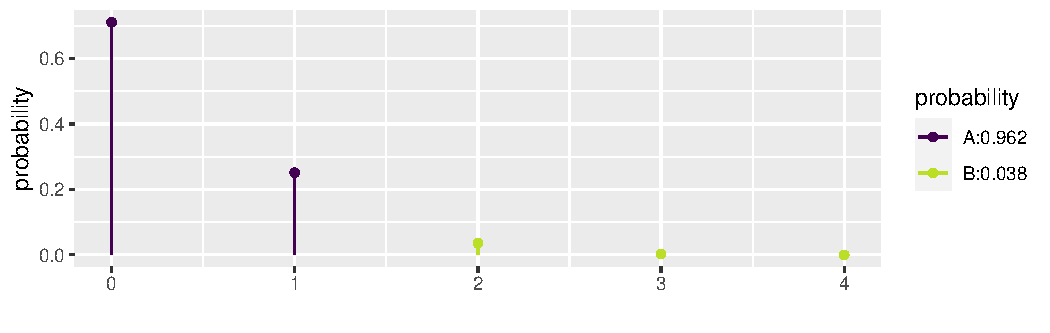
\includegraphics[width=\maxwidth]{figure/unnamed-chunk-12-1} 

}


\begin{kframe}\begin{verbatim}
## [1] 0.038
\end{verbatim}
\end{kframe}
\end{knitrout}
	
\end{frame}



\section{Inference concerning a proportion $\pi$, based on s.r.s. of size $n$}



\begin{frame}{Examples}
	\small 
	The \textbf{Parameter} $\pi$ of interest: the proportion ...
	\begin{itemize}
		\item with undiagnosed hypertension / seeing MD during a 1-year span 
		\item who would respond to a specific therapy 
		\item still breast-feeding at 6 months
		\item of pairs where response on treatment $>$  response on placebo
		\item of Earth's surface covered by water
		\item who \textit{would} enrol in a long-term study or answer a questionnaire
		\item of twin pairs where left-handed twin dies first
		\item able to tell imported from domestic beer in a ``triangle taste test''
	\end{itemize}
	
	Inference via \textbf{Statistic}: the number ($y$) or proportion $p = y/n$ `positive' in an s.r.s. of size $n$.
	
\end{frame}


\begin{comment}
\begin{frame}{Frequentist vs. Bayesian Inference}
\small 
\Wider[5em]{
\begin{tabular}{ll}
\textbf{Frequentist ($\S 2.1$}) & \textbf{Bayesian  ($\S 2.2$)} \\
& \\
- based on prob[ data $| \theta$ ], i.e. & - based on prob[ $\theta | $data ], i.e.,  \\
- probability statements about data & - probability statements about $\pi $  \\
& \\
Evidence (P-value) against $H_{0}$: $\pi = \pi_{0}$ & - point estimate: \\
& mean/median/mode of  \\
Test of H$_{0}$: Is P-value $<$ (preset) $\alpha$? & posterior distribution of $\pi$ \\
CI:  interval estmate & - (credible) interval  \\ 
\end{tabular}
}
\end{frame}
\end{comment}



\begin{frame}
	\Wider[5em]{
		
		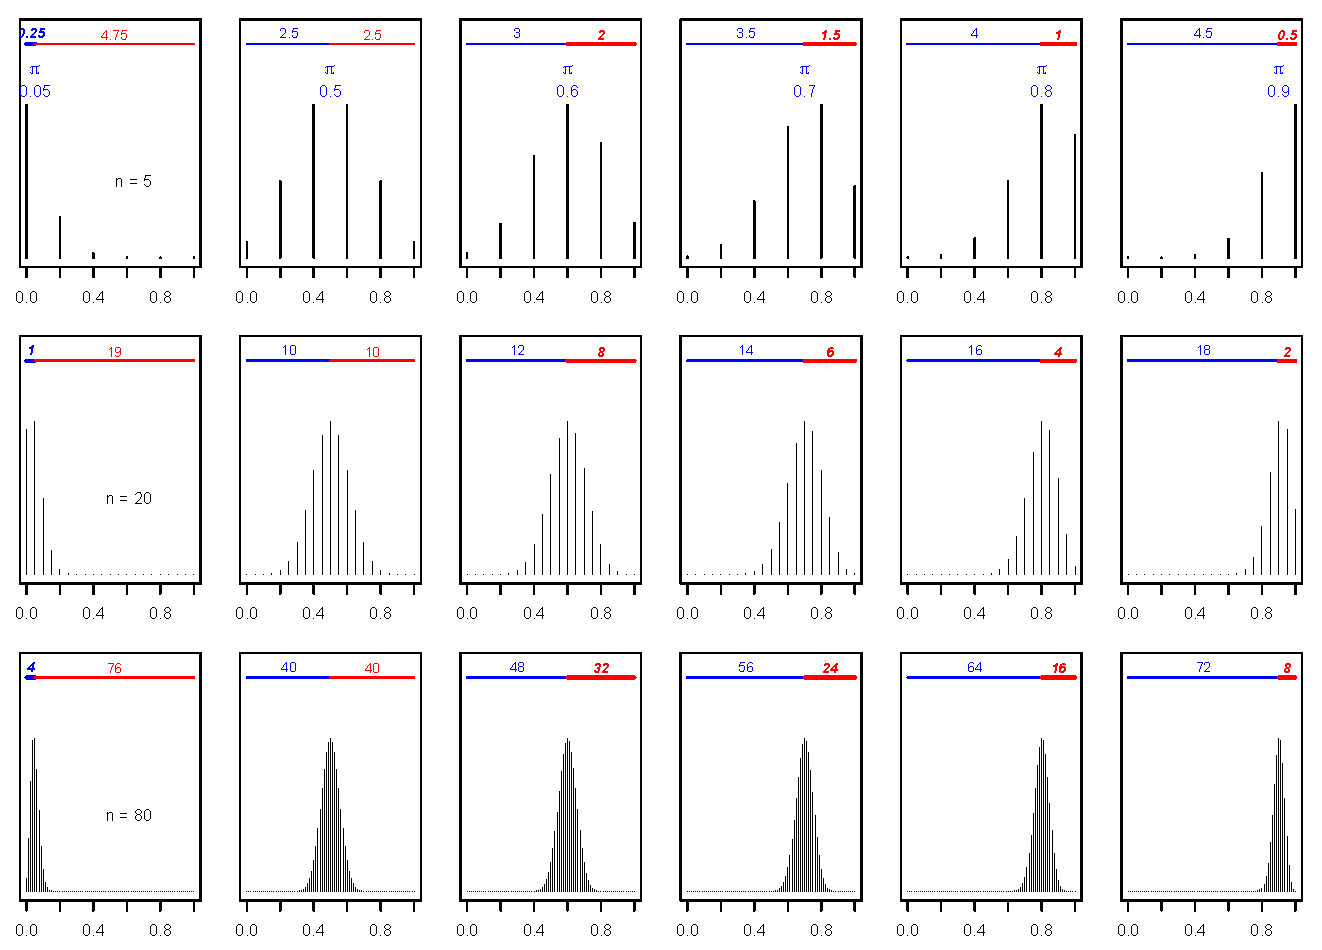
\includegraphics[width=4.95in,height=3.7in]{BinomialsVarious.pdf}
		
		
	}
\end{frame}



\begin{frame}{Justification for the $n \times \pi$ and $n \times (1-\pi)$ $\geq 10$ }
	notes on the Figure from the previous slide:
	\begin{itemize}
		\setlength\itemsep{1em}
		\item \textbf{Binomial distributions}, on (0,1) scale (rather than \texttt{0:n}). Bigger  expected numbers of { \color{blue}{`\textbf{positives}'} } \textbf{\underline{and}} { \color{red}{`\textbf{negatives}'}} imply less probability mass at the extreme(s) and thus help to approximate the (binomial) sampling distribution by a Gaussian distribution with mean $\pi$ and 
		$\sigma = \frac{ \{\pi(1-\pi)\}^{1/2}}{\sqrt{n}}.$
		\item The amount of space needed at each extreme in order to accommodate a Gaussian distribution that does not spill over beyond the (0,1) boundaries is just another way to explain the (`taught but not explained')  rule-of-thumb that the expected numbers, $n \times \pi$ and $n \times (1-\pi)$ should should exceed 10 
	\end{itemize}
\end{frame}


\section{Frequentist Confidence Interval for $\pi$, based on an observed proportion $p = y/n$ \texttt{stats::binom.test} and \texttt{mosaic::binom.test} in \texttt{R}}


\begin{frame}{Some background}
	\small
	
	\begin{itemize}
		\item \underline{It is sad} that even today, with more emphasis on CI's and less on p-values and tests, we have to go through the `\texttt{.test}' to get to the CI. It is also of note that the procedure mentions the model (binomial) rather than the target parameter, the proportion $\pi.$ 
		
		\item The base \texttt{stats::binom.test} function in \texttt{R} has just one method, the Clopper-Pearson one. The \texttt{mosaic::binom.test} one has it and four others, and these allow us to appreciate why different ones might be used in different circumstances. We will start with the most familiar of them, the so-called `Wald' CI, which, because of its `point estimate $\pm \textrm{Margin.Of.Error}$' form, is \textit{symmetric}. 
		
		\item The \texttt{mosaic::binom.test} allows for a vector of individual 0's and 1's, rather than the tallies of 1's and 0's required for \texttt{stats::binom.test} 
		
		\pause
		
		\item In practice, \textbf{CIs for proportions, and functions thereof, will come from regression models}. 
		
	\end{itemize}
\end{frame}


\begin{frame}{CI based on Gaussian approximation to sampling distribution of the sample proportion $p$ -- the `Wald' method in \texttt{mosaic::binom.test}}
	\begin{center}
	\begin{figure}
		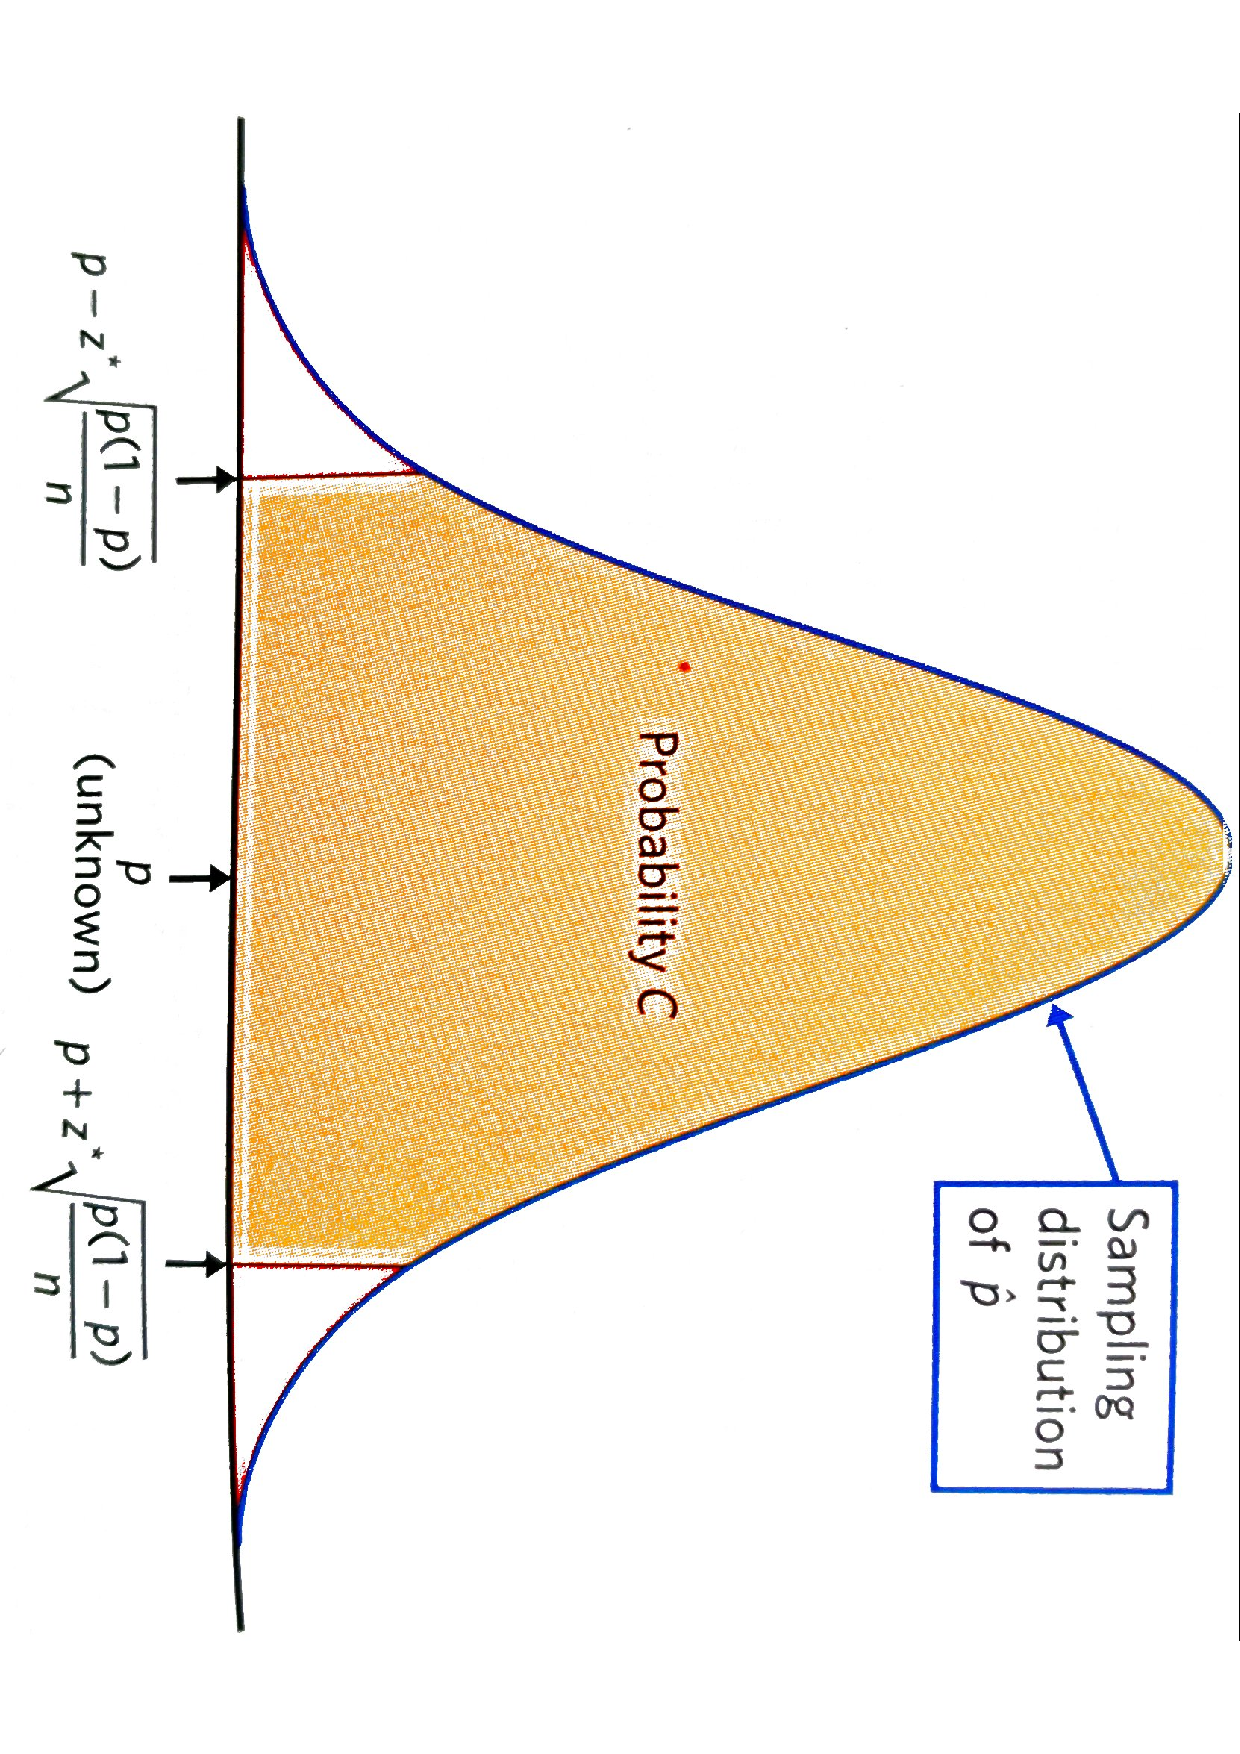
\includegraphics[scale=0.3,angle=90]{prop1.pdf}
	\end{figure}
\end{center}
	
\end{frame}




\begin{frame}{CI based on Normal approximation to sampling distribution of the sample proportion $p$ -- the `Wald' method in \texttt{mosaic::binom.test}}
	\small
	\begin{itemize}
		\item Dividing this $\widehat{\sigma_{0/1}}$ by the square root of $n$, we get the standard error, our best estimate of the spread of the sampling distribution of a sample proportion, i.e.,
		$$SE[p] = \frac{\sqrt{p(1-p)}}{\sqrt{n}} \ \ \ \  \ = \ \frac{\widehat{\sigma_{0/1}}}{\sqrt{n}} \  .$$ 
		\item So, as it is \underline{traditionally} presented,  the CI becomes
		$$p \  \pm  \ z^\star \times \sqrt{\frac{p(1-p)}{n}}.$$ 
		\item As we will see below, now that we seldom calculate a CI `from scratch,'  \underline{today} the Wald CI is better presented in the \underline{\texttt{R-computational} form}
		\scriptsize{$$\texttt{qnorm(p=c(0.025,0.975),  mean= p,  sd = sqrt(p*(1-p))/sqrt(n))}.$$}
	\end{itemize}
\end{frame}




\begin{frame}[fragile]{Example 1: Assessing the prevalence of HPV infections}
	\small
	NHANES found that 515 of a sample of 1921 women aged 14 to 59 years currently tested positive for HPV. Provide a 99\% confidence interval for HPV prevalence. 
	
\begin{knitrout}\tiny
\definecolor{shadecolor}{rgb}{0.969, 0.969, 0.969}\color{fgcolor}\begin{kframe}
\begin{alltt}
\hlstd{n} \hlkwb{<-} \hlnum{1921}
\hlstd{number_infected} \hlkwb{<-} \hlnum{515}
\hlstd{p} \hlkwb{<-} \hlstd{number_infected} \hlopt{/} \hlstd{n}
\hlstd{s} \hlkwb{<-} \hlkwd{sqrt}\hlstd{(p} \hlopt{*} \hlstd{(}\hlnum{1} \hlopt{-} \hlstd{p))}
\hlstd{SEP} \hlkwb{<-} \hlstd{s} \hlopt{/} \hlkwd{sqrt}\hlstd{(n)}
\hlstd{mosaic}\hlopt{::}\hlkwd{xqnorm}\hlstd{(}\hlkwc{p}\hlstd{=}\hlkwd{c}\hlstd{(}\hlnum{0.005}\hlstd{,}\hlnum{0.995}\hlstd{),} \hlkwc{mean} \hlstd{= p,} \hlkwc{sd} \hlstd{= SEP)}
\end{alltt}
\end{kframe}

{\centering 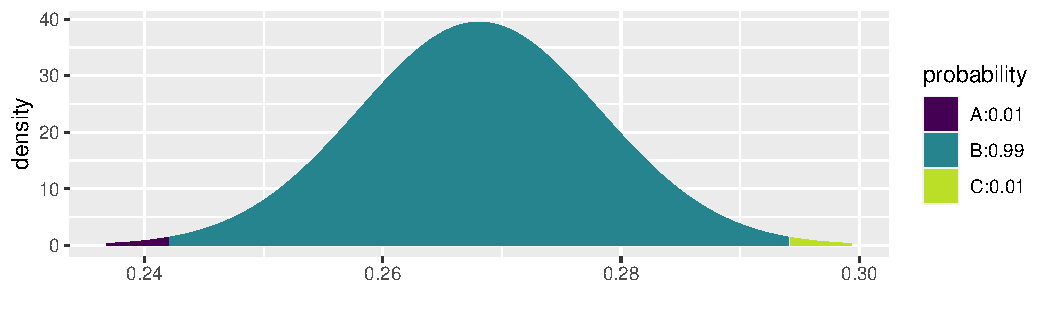
\includegraphics[width=\maxwidth]{figure/unnamed-chunk-13-1} 

}


\begin{kframe}\begin{verbatim}
## [1] 0.24 0.29
\end{verbatim}
\end{kframe}
\end{knitrout}
	
\end{frame}


\begin{frame}[fragile]{Example 2: Assessing the prevalence of HPV infections}
	
\begin{knitrout}\tiny
\definecolor{shadecolor}{rgb}{0.969, 0.969, 0.969}\color{fgcolor}\begin{kframe}
\begin{alltt}
\hlstd{mosaic}\hlopt{::}\hlkwd{binom.test}\hlstd{(}\hlkwc{x} \hlstd{=} \hlnum{515}\hlstd{,} \hlkwc{n} \hlstd{=} \hlnum{1921}\hlstd{,} \hlkwc{ci.method}\hlstd{=}\hlkwd{c}\hlstd{(}\hlstr{"wald"}\hlstd{),} \hlkwc{conf.level}\hlstd{=}\hlnum{0.99}\hlstd{)}
\end{alltt}
\begin{verbatim}
## Exact binomial test (Wald CI) with 515 out of 1921 
## number of successes = 515, number of trials = 1921, p-value < 2.2e-16
## alternative hypothesis: true probability of success is not equal to 0.5 
## 99 percent confidence interval:
##  0.24 0.29 
## sample estimates:
## probability of success 
##                   0.27
\end{verbatim}
\end{kframe}
\end{knitrout}
	Note: HPV positive $\ne$ `success' !!
\end{frame}



\begin{frame}[fragile]{Example 2: Proportion of Earth Covered by Water}
	
	Suppose our observed proportion of `water' locations was $p = 4/5,$ or 80\%.
	
\begin{knitrout}\tiny
\definecolor{shadecolor}{rgb}{0.969, 0.969, 0.969}\color{fgcolor}\begin{kframe}
\begin{alltt}
\hlstd{mosaic}\hlopt{::}\hlkwd{binom.test}\hlstd{(}\hlkwc{x} \hlstd{=} \hlnum{4}\hlstd{,} \hlkwc{n} \hlstd{=} \hlnum{5}\hlstd{,} \hlkwc{ci.method}\hlstd{=}\hlkwd{c}\hlstd{(}\hlstr{"wald"}\hlstd{),} \hlkwc{conf.level}\hlstd{=}\hlnum{0.95}\hlstd{)}
\end{alltt}
\begin{verbatim}
## Exact binomial test (Wald CI) with 4 out of 5 
## number of successes = 4, number of trials = 5, p-value = 0.375
## alternative hypothesis: true probability of success is not equal to 0.5 
## 95 percent confidence interval:
##  0.45 1.15 
## sample estimates:
## probability of success 
##                    0.8
\end{verbatim}
\end{kframe}
\end{knitrout}
	
	\pause 
	
	Clearly  the proportion or percentage of the Earth's surface covered by water cannot
	be \underline{1.15} or \underline{115}\%.  
	
\end{frame}


\begin{frame}[fragile]{Example 2: Proportion of Earth Covered by Water}
	
\begin{knitrout}\tiny
\definecolor{shadecolor}{rgb}{0.969, 0.969, 0.969}\color{fgcolor}\begin{kframe}
\begin{alltt}
\hlstd{stats}\hlopt{::}\hlkwd{qnorm}\hlstd{(}\hlkwc{p}\hlstd{=}\hlkwd{c}\hlstd{(}\hlnum{0.025}\hlstd{,}\hlnum{0.975}\hlstd{),} \hlkwc{mean} \hlstd{=} \hlnum{0}\hlstd{,} \hlkwc{sd} \hlstd{=} \hlkwd{sqrt}\hlstd{(}\hlnum{0} \hlopt{*} \hlnum{1} \hlopt{/} \hlnum{5}\hlstd{))}
\end{alltt}
\begin{verbatim}
## [1] 0 0
\end{verbatim}
\begin{alltt}
\hlstd{stats}\hlopt{::}\hlkwd{qnorm}\hlstd{(}\hlkwc{p}\hlstd{=}\hlkwd{c}\hlstd{(}\hlnum{0.025}\hlstd{,}\hlnum{0.975}\hlstd{),} \hlkwc{mean} \hlstd{=} \hlnum{0.2}\hlstd{,} \hlkwc{sd} \hlstd{=} \hlkwd{sqrt}\hlstd{(}\hlnum{0.2} \hlopt{*} \hlnum{0.8} \hlopt{/} \hlnum{5}\hlstd{))}
\end{alltt}
\begin{verbatim}
## [1] -0.15  0.55
\end{verbatim}
\begin{alltt}
\hlstd{stats}\hlopt{::}\hlkwd{qnorm}\hlstd{(}\hlkwc{p}\hlstd{=}\hlkwd{c}\hlstd{(}\hlnum{0.025}\hlstd{,}\hlnum{0.975}\hlstd{),} \hlkwc{mean} \hlstd{=} \hlnum{0.4}\hlstd{,} \hlkwc{sd} \hlstd{=} \hlkwd{sqrt}\hlstd{(}\hlnum{0.4} \hlopt{*} \hlnum{0.6} \hlopt{/} \hlnum{5}\hlstd{))}
\end{alltt}
\begin{verbatim}
## [1] -0.029  0.829
\end{verbatim}
\begin{alltt}
\hlstd{stats}\hlopt{::}\hlkwd{qnorm}\hlstd{(}\hlkwc{p}\hlstd{=}\hlkwd{c}\hlstd{(}\hlnum{0.025}\hlstd{,}\hlnum{0.975}\hlstd{),} \hlkwc{mean} \hlstd{=} \hlnum{0.6}\hlstd{,} \hlkwc{sd} \hlstd{=} \hlkwd{sqrt}\hlstd{(}\hlnum{0.6} \hlopt{*} \hlnum{0.4} \hlopt{/} \hlnum{5}\hlstd{))}
\end{alltt}
\begin{verbatim}
## [1] 0.17 1.03
\end{verbatim}
\begin{alltt}
\hlstd{stats}\hlopt{::}\hlkwd{qnorm}\hlstd{(}\hlkwc{p}\hlstd{=}\hlkwd{c}\hlstd{(}\hlnum{0.025}\hlstd{,}\hlnum{0.975}\hlstd{),} \hlkwc{mean} \hlstd{=} \hlnum{0.8}\hlstd{,} \hlkwc{sd} \hlstd{=} \hlkwd{sqrt}\hlstd{(}\hlnum{0.8} \hlopt{*} \hlnum{0.2} \hlopt{/} \hlnum{5}\hlstd{))}
\end{alltt}
\begin{verbatim}
## [1] 0.45 1.15
\end{verbatim}
\begin{alltt}
\hlstd{stats}\hlopt{::}\hlkwd{qnorm}\hlstd{(}\hlkwc{p}\hlstd{=}\hlkwd{c}\hlstd{(}\hlnum{0.025}\hlstd{,}\hlnum{0.975}\hlstd{),} \hlkwc{mean} \hlstd{=} \hlnum{1}\hlstd{,} \hlkwc{sd} \hlstd{=} \hlkwd{sqrt}\hlstd{(}\hlnum{1} \hlopt{*} \hlnum{0} \hlopt{/} \hlnum{5}\hlstd{))}
\end{alltt}
\begin{verbatim}
## [1] 1 1
\end{verbatim}
\end{kframe}
\end{knitrout}
	
	
\end{frame}



\begin{frame}{Example 2: Proportion of Earth Covered by Water}
	Thus, \textbf{\underline{whatever your result}}, the Wald 95\% CI gives a \textit{\textbf{nonsensical}} result. Using the Normal/Gaussian approximation to the Binomial sampling distribution does not work when $n=5.$
\end{frame}


\section{What to do if a symmetric Gaussian-based CI doesn't make sense?}


\begin{frame}{What to do if a symmetric Gaussian-based CI doesn't make sense?}
	\begin{itemize}
		\setlength\itemsep{1em}
		\item \textbf{Answer}: use a non-symmetric one, and one that respects the (0,1) scale. \pause 
		\item The other 4 methods in \texttt{mosaic::binom.test} do respect the (0,1) scale \pause 
		\item We can also switch to the ($-\infty, \infty$)  \textit{logit} scale, computing the CI in this scale, and then back-transforming to the (0,1) scale $\to$ logistic regression.
	\end{itemize}
\end{frame}



\begin{frame}{1. Asymmetric (Wilson and Clopper-Pearson) Methods}
	\small
	\begin{itemize}
		\setlength\itemsep{1em}
		\item The text in the next Figure is a shortened, more concrete, and more modern version of what Wilson wrote in 1927. He began by saying that by adding (symmetric) margins of error to the point estimate,
		the usual method up to then (and still today) gives the wrong impression that the truth varies around the point estimate when in fact \underline{it is the point estimate that varies around the truth !!} 
		
		\item So, he suggests that we should reverse our logic and ask under what worst case scenarios  involving the truth would we have observed (such) an extreme point estimate.
		
		
	\end{itemize}
\end{frame}


\begin{frame}{1. Asymmetric (Wilson and Clopper-Pearson) Methods}
	\small
	\begin{itemize}
		\setlength\itemsep{.71em}
		\item We begin with one of these scenarios, say the one where the point estimate lands to the right of (is above) the truth. \underline{By trial and error} we can find a lower value for the truth, namely $\pi_{Lower},$ such that the observed value would be a over-estimate, located at the 97.5\%ile. 
		
		\item Then we consider the reverse scenario, and we find a value for the truth, namely $\pi_{Upper},$ such that the observed value would be an under-estimate, located at the 2.5\%ile. 
		
		\item Since the sampling distributions at $\pi = \pi_{Lower}$ and $\pi = \pi_{Upper}$ may well have very different shapes and widths, the observed proportion, p, will not be equidistant from $\pi = \pi_{Lower}$ and $\pi = \pi_{Upper}.$
	\end{itemize}
\end{frame}


\begin{frame}
\begin{knitrout}\tiny
\definecolor{shadecolor}{rgb}{0.969, 0.969, 0.969}\color{fgcolor}

{\centering 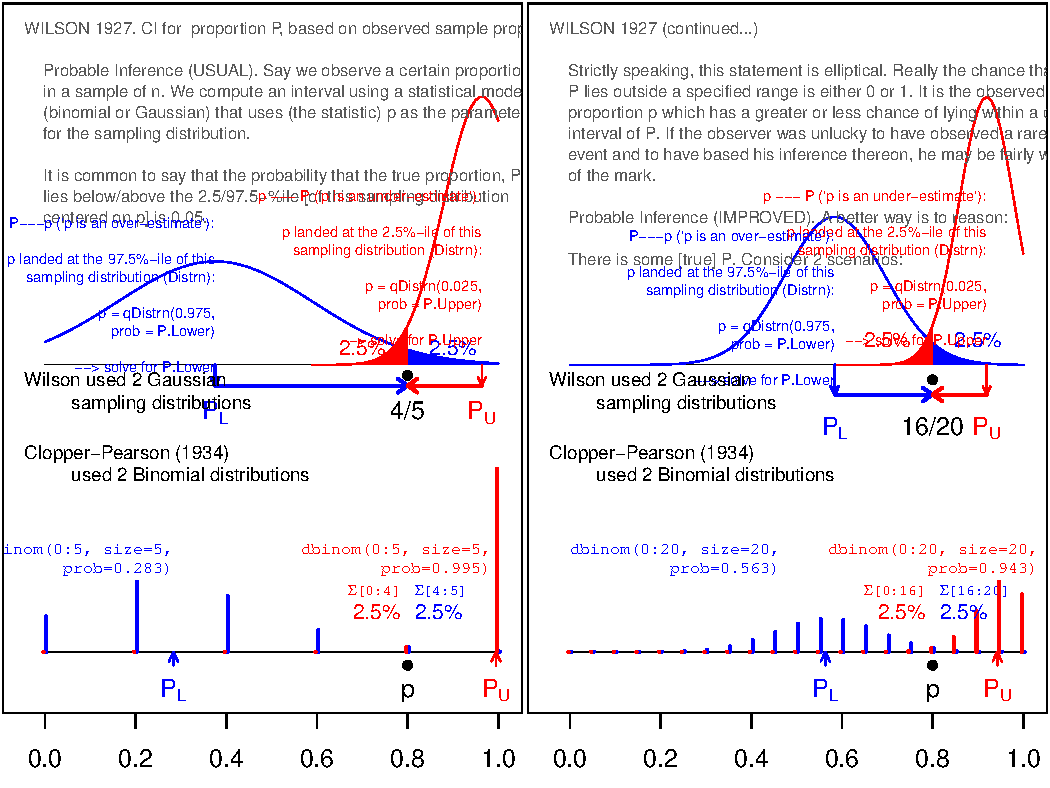
\includegraphics[width=\maxwidth]{figure/wilson-1} 

}



\end{knitrout}
\end{frame}


\begin{frame}[fragile]{Clopper-Pearson 95\% CI when $p = 4/5$}
\begin{knitrout}\tiny
\definecolor{shadecolor}{rgb}{0.969, 0.969, 0.969}\color{fgcolor}\begin{kframe}
\begin{alltt}
\hlcom{# upper limit --> lower tail needs 2.5%}
\hlstd{manipulate}\hlopt{::}\hlkwd{manipulate}\hlstd{(}
\hlstd{mosaic}\hlopt{::}\hlkwd{xpbinom}\hlstd{(}\hlnum{4}\hlstd{,} \hlkwc{size} \hlstd{=} \hlnum{5}\hlstd{,} \hlkwc{prob} \hlstd{= proba),}
\hlkwc{proba} \hlstd{= manipulate}\hlopt{::}\hlkwd{slider}\hlstd{(}\hlnum{0.001}\hlstd{,} \hlnum{0.999}\hlstd{,} \hlkwc{step} \hlstd{=} \hlnum{0.001}\hlstd{))}

\hlcom{# lower limit --> upper tail needs 2.5%}
\hlcom{# when lower.tail=FALSE, pbinom doesnt include k, i.e., P(Y > k)}
\hlstd{manipulate}\hlopt{::}\hlkwd{manipulate}\hlstd{(}
\hlstd{mosaic}\hlopt{::}\hlkwd{xpbinom}\hlstd{(}\hlnum{3}\hlstd{,} \hlkwc{size} \hlstd{=} \hlnum{5}\hlstd{,} \hlkwc{prob} \hlstd{= proba,} \hlkwc{lower.tail} \hlstd{=} \hlnum{FALSE}\hlstd{),}
\hlkwc{proba} \hlstd{= manipulate}\hlopt{::}\hlkwd{slider}\hlstd{(}\hlnum{0.001}\hlstd{,} \hlnum{0.999}\hlstd{,} \hlkwc{step} \hlstd{=} \hlnum{0.001}\hlstd{))}
\end{alltt}
\end{kframe}
\end{knitrout}
	
	\blue{Question:} Should the interval be different when $p=16/20=0.8 = 4/5$?
\end{frame}


\begin{frame}[fragile]{Clopper-Pearson 95\% CI when $p = 16/20$}
\begin{knitrout}\tiny
\definecolor{shadecolor}{rgb}{0.969, 0.969, 0.969}\color{fgcolor}\begin{kframe}
\begin{alltt}
\hlcom{# upper limit --> lower tail needs 2.5%}
\hlstd{manipulate}\hlopt{::}\hlkwd{manipulate}\hlstd{(}
\hlstd{mosaic}\hlopt{::}\hlkwd{xpbinom}\hlstd{(}\hlnum{16}\hlstd{,} \hlkwc{size} \hlstd{=} \hlnum{20}\hlstd{,} \hlkwc{prob} \hlstd{= proba),}
\hlkwc{proba} \hlstd{= manipulate}\hlopt{::}\hlkwd{slider}\hlstd{(}\hlnum{0.001}\hlstd{,} \hlnum{0.999}\hlstd{,} \hlkwc{step} \hlstd{=} \hlnum{0.001}\hlstd{))}


\hlcom{# lower limit --> upper tail needs 2.5%}
\hlstd{manipulate}\hlopt{::}\hlkwd{manipulate}\hlstd{(}
\hlstd{mosaic}\hlopt{::}\hlkwd{xpbinom}\hlstd{(}\hlnum{15}\hlstd{,} \hlkwc{size} \hlstd{=} \hlnum{20}\hlstd{,} \hlkwc{prob} \hlstd{= proba,} \hlkwc{lower.tail} \hlstd{=} \hlnum{FALSE}\hlstd{),}
\hlkwc{proba} \hlstd{= manipulate}\hlopt{::}\hlkwd{slider}\hlstd{(}\hlnum{0.001}\hlstd{,} \hlnum{0.999}\hlstd{,} \hlkwc{step} \hlstd{=} \hlnum{0.001}\hlstd{))}
\end{alltt}
\end{kframe}
\end{knitrout}
\end{frame}


\begin{frame}[fragile]{Clopper-Pearson 95\% CI in R}
\begin{knitrout}\tiny
\definecolor{shadecolor}{rgb}{0.969, 0.969, 0.969}\color{fgcolor}\begin{kframe}
\begin{alltt}
\hlstd{mosaic}\hlopt{::}\hlkwd{binom.test}\hlstd{(}\hlkwc{x}\hlstd{=}\hlnum{4}\hlstd{,} \hlkwc{n}\hlstd{=}\hlnum{5}\hlstd{,} \hlkwc{ci.method}\hlstd{=}\hlkwd{c}\hlstd{(}\hlstr{"Clopper-Pearson"}\hlstd{))}
\end{alltt}
\begin{verbatim}
##  with 4 out of 5 
## number of successes = 4, number of trials = 5, p-value = 0.375
## alternative hypothesis: true probability of success is not equal to 0.5 
## 95 percent confidence interval:
##  0.28 0.99 
## sample estimates:
## probability of success 
##                    0.8
\end{verbatim}
\begin{alltt}
\hlstd{mosaic}\hlopt{::}\hlkwd{binom.test}\hlstd{(}\hlkwc{x}\hlstd{=}\hlnum{16}\hlstd{,} \hlkwc{n}\hlstd{=}\hlnum{20}\hlstd{,} \hlkwc{ci.method}\hlstd{=}\hlkwd{c}\hlstd{(}\hlstr{"Clopper-Pearson"}\hlstd{))}
\end{alltt}
\begin{verbatim}
##  with 16 out of 20 
## number of successes = 16, number of trials = 20, p-value = 0.01182
## alternative hypothesis: true probability of success is not equal to 0.5 
## 95 percent confidence interval:
##  0.56 0.94 
## sample estimates:
## probability of success 
##                    0.8
\end{verbatim}
\end{kframe}
\end{knitrout}
\end{frame}


\begin{frame}{Binomial-based (95\%) CIs for $\pi$ using a nomogram}
	\small
	\begin{itemize}
		\setlength\itemsep{.11em}
		\item The panels in the next Figure present binomial-based (95\%) CIs for a proportion
		using the `nomogram' format introduced by Clopper and Pearson -- but using
		the Wilson method to compute them. 
		\item  \textit{\textbf{Example}}: in the case of an observed proportion of  say 16/20 = 0.8, the Nomogram yields a 95\% CI of 56.3\% (solid  square located above p=0.8, on the innermost -- [n = 20] -- blue band) to 94.3\% (solid circle located at the same p on the innermost -- [n  = 20] -- red band). 
		
		\item Read \textbf{horizontally}, the nomogram shows the variability of proportions from s.r.s samples of size $n$. Read \textbf{vertically}, it shows: (i) CI $\rightarrow$ symmetry as $p \rightarrow 0.5$ or  $n \nearrow $ [in fact, as  $n \times p \  \textrm{and} \ n(1 - p) \nearrow $ \ ]
		(ii) the widest ME's are at $p=0.5;$ thus, they can be used as the `widest ME' scenario.
		
		\item The next chart shows what $n$ will give a desired margin of error. It also shows the `\textit{quadruple the effort to halve the uncertainty}' rule. And -- at their widest -- how wide the ME's are for various values of $n.$
	\end{itemize}
\end{frame}


\begin{frame}
	\Wider[5em]{	
		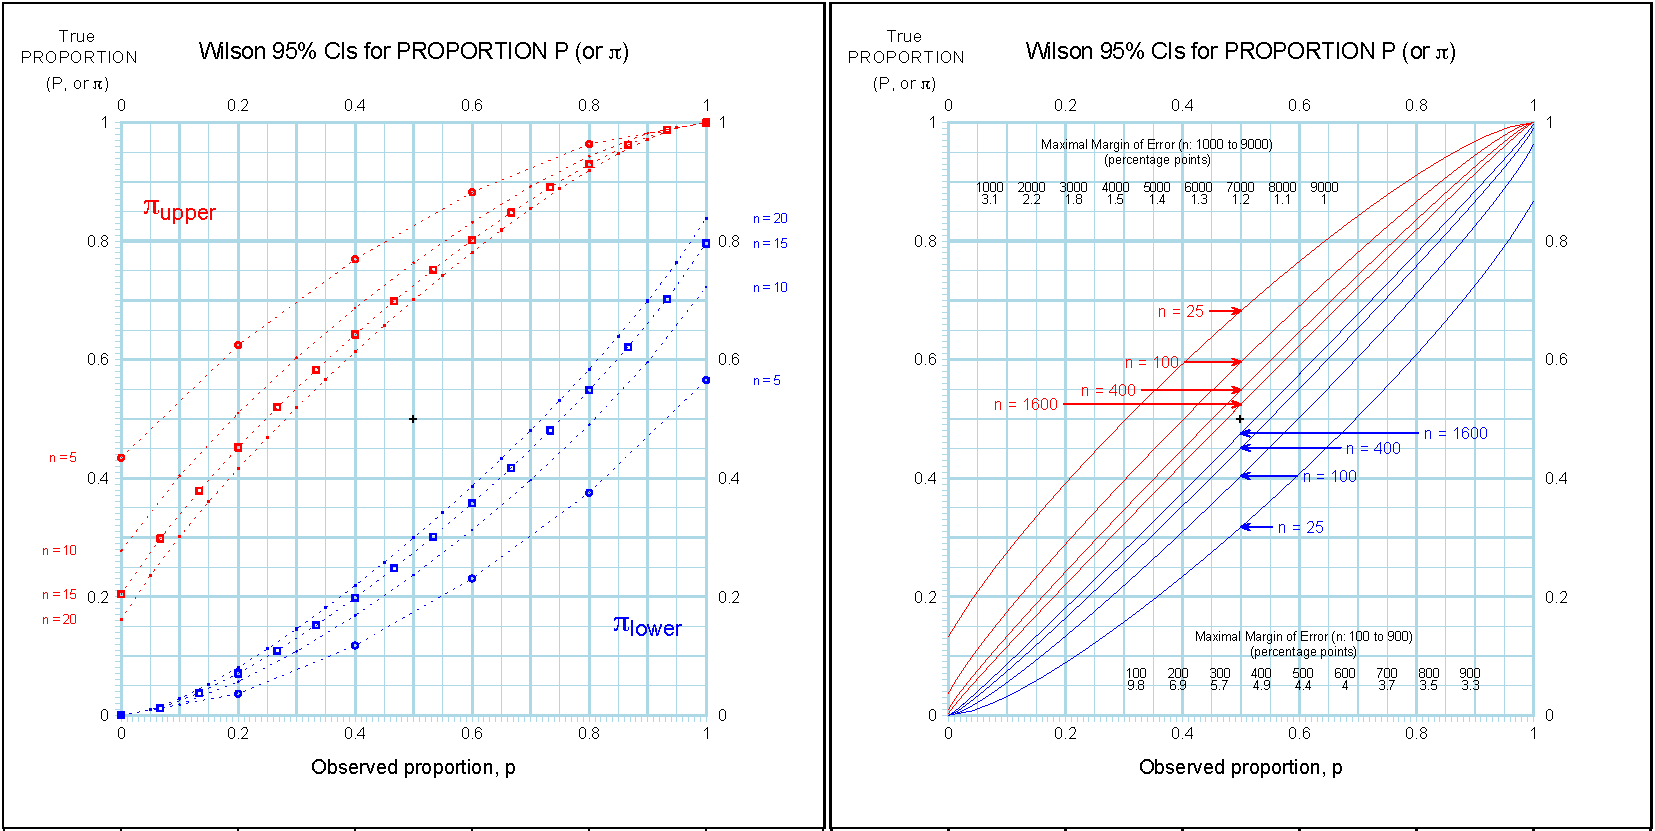
\includegraphics[width=4.95in,height=3.6in]{Nomogram.pdf}
	}
\end{frame}

\begin{frame}{2. Add 2 to numerator, 4 to denominator rule}
	\small
	\begin{itemize}
		\setlength\itemsep{1em}
		\item The confidence interval  $\hat{p} \pm z \sqrt{\hat{p}(1-\hat{p})/n}$ for $\pi$ is easy
		to calculate. It is also easy to understand, because it rests directly on the approximately Normal distribution of $p.$ 
		\item Unfortunately, confidence levels from this interval are often quite inaccurate unless the sample is very large. Simulations show that the actual confidence level is usually less than the confidence level you asked for in choosing the critical value $z$. That's bad. 
		\item What is worse, accuracy does not consistently get better as the sample size n increases. There are ``lucky'' and ``unlucky'' combinations of the sample size $n$ and the true population proportion $p.$ 
		
		
	\end{itemize}
\end{frame}



\begin{frame}{2. Add 2 to numerator, 4 to denominator rule}
	\small
	\begin{itemize}
		\setlength\itemsep{1em}
		
		\item Fortunately, there is a simple modification that has been shown experimentally
		to successfully improve the accuracy of the confidence interval. We call it the ``plus
		four'' method, because all you need to do is \textit{add four imaginary observations, 
			two successes and two failures}. With the added observations, the plus four estimate of $\pi$ is
		$$\widetilde{p} =\frac{\textrm{number of `positives' in the sample} + 2}{n+4}$$ 
		
		\item \underline{The formula for the confidence interval is exactly as before}, with the new sample
		size and number of `positives.' You do not need software that offers the plus four
		interval - just enter the new sample size (actual size + 4) and number of `positives'
		into the large-sample procedure.
	\end{itemize}
\end{frame}


\begin{frame}{3. 95\% CI for $\pi$ using a transformation of scale}
	
	\begin{itemize}
		\item Based on \textbf{Gaussian distribution of the \underline{logit} \underline{transformation}} of  the point estimate ($p$, the observed proportion) and of  the parameter $\pi.$
	\end{itemize}
	
	\small
	\textbf{Parameter: \footnote{UPPER CASE / Greek = parameter; lower case / Roman = statistic.} }
	
	logit$\{ \pi \}$
	= log$\{ ODDS \}$ \footnote{Here, $\textrm{log} = `natural'$ log, i.e. to base e, which some write as $\ln.$} 
	=   log$\big\{ \frac{\pi}{(1-\pi)} \big\}$ 
	=  log$ \big\{ \frac{ \textrm{PROPORTION ``Positive''} }
	{ \textrm{PROPORTION ``Negative''} } \big\}$ \\
	
	\textbf{Statistic: } logit$\{ p \}$
	= log$\{ odds \}$ 
	=  log$ \big\{ \frac{ \textrm{proportion ``Positive''} }
	{ \textrm{proportion ``Negative''} } \big\}.$ \\ \ \\
	
	\textbf{Reverse transformation} (to get back from LOGIT to $\pi $) ...
	$$\pi = \frac{\textrm{ODDS}}{1 + \textrm{ODDS}} = \frac{\exp [LOGIT]}{1 + \exp[LOGIT]}.$$
	likewise...
	$$p = \frac{odds}{1 \textrm{ }+ \textrm{ }odds} = \frac{\exp [logit]}{1\textrm{ }+\textrm{ }\exp [logit]}.$$
	
	
\end{frame}

\begin{frame}{3. 95\% CI for $\pi$ using a transformation of scale}
	\small
	
	$\pi _{LOWER} = \frac{\exp \{\textrm{LOWER limit of LOGIT}\}}{1 + \exp \{\textrm{LOWER limit of LOGIT}\}} 
	=\frac{\exp \{logit - z_{\alpha/2}SE[logit]\}}{1 + \exp \{logit - z_{\alpha/2}SE[logit]\}} $ \\ \ \\
	
	$\pi _{UPPER}$ likewise.  \\ \ \\
	
	$SE[logit] = \big\{ \frac{1}{\# \textrm{ positive} }
	+ \frac{1}{\# \textrm{ negative} }
	\big\}^{1/2}$ \\ \ \\
	
	
	
	\begin{itemize}
		\item $p = 16/20 \Rightarrow odds = 16/4 \Rightarrow  logit = \log[16/4] = 1.386.$ 
		
		\item $SE[logit] =\{1/16 + 1/4 \}^{1/2} = 0.559$ 
		
		\item $  \Rightarrow \textrm{95\% CI in LOGIT[}\pi] \textrm{ scale: } 1.386 \pm 1.96\times 0.559
		= \{0.290, 2.482\}$ \footnote{  
			\texttt{qnorm(p=c(0.025,0.975), mean=log(16/4), sd=sqrt(1/16+1/4))}: 0.290 to 2.482.}
		
		\item $ \Rightarrow \textrm{CI in } \pi \textrm{ scale: }  \{ \exp(0.290)/(1+\exp(0.290), \
		\exp(2.482)/(1+\exp(2.482) \}$ 
	\end{itemize}
	
\end{frame}


\begin{frame}[fragile]{4. 95\% CI for $\pi$ using logistic regression}
	
\begin{knitrout}\tiny
\definecolor{shadecolor}{rgb}{0.969, 0.969, 0.969}\color{fgcolor}\begin{kframe}
\begin{alltt}
\hlstd{fit} \hlkwb{<-} \hlkwd{glm}\hlstd{(}\hlkwd{cbind}\hlstd{(}\hlnum{16}\hlstd{,}\hlnum{4}\hlstd{)} \hlopt{~} \hlnum{1}\hlstd{,} \hlkwc{family}\hlstd{=binomial)}
\end{alltt}
\end{kframe}
\end{knitrout}
	
% latex table generated in R 4.0.2 by xtable 1.8-4 package
% Wed Nov  4 10:56:42 2020
\begin{table}[ht]
\centering
\begin{tabular}{rrrrr}
  \hline
 & Estimate & Std. Error & z value & Pr($>$$|$z$|$) \\ 
  \hline
(Intercept) & 1.3863 & 0.5590 & 2.48 & 0.0131 \\ 
   \hline
\end{tabular}
\end{table}

	
\begin{knitrout}\tiny
\definecolor{shadecolor}{rgb}{0.969, 0.969, 0.969}\color{fgcolor}\begin{kframe}
\begin{alltt}
\hlkwd{plogis}\hlstd{(fit}\hlopt{$}\hlstd{coef[}\hlnum{1}\hlstd{])}
\end{alltt}
\begin{verbatim}
## (Intercept) 
##         0.8
\end{verbatim}
\begin{alltt}
\hlkwd{round}\hlstd{(}\hlkwd{plogis}\hlstd{(}\hlkwd{confint}\hlstd{(fit)),}\hlnum{2}\hlstd{)}
\end{alltt}
\begin{verbatim}
##  2.5 % 97.5 % 
##   0.59   0.93
\end{verbatim}
\end{kframe}
\end{knitrout}
	
\end{frame}



\begin{frame}[fragile]{Session Info}
	\tiny
	
\begin{knitrout}\tiny
\definecolor{shadecolor}{rgb}{0.969, 0.969, 0.969}\color{fgcolor}\begin{kframe}
\begin{verbatim}
R version 4.0.2 (2020-06-22)
Platform: x86_64-pc-linux-gnu (64-bit)
Running under: Pop!_OS 20.04 LTS

Matrix products: default
BLAS:   /usr/lib/x86_64-linux-gnu/openblas-pthread/libblas.so.3
LAPACK: /usr/lib/x86_64-linux-gnu/openblas-pthread/liblapack.so.3

attached base packages:
[1] tools     stats     graphics  grDevices utils     datasets  methods  
[8] base     

other attached packages:
 [1] NCStats_0.4.7   FSA_0.8.30      forcats_0.5.0   stringr_1.4.0  
 [5] dplyr_1.0.2     purrr_0.3.4     readr_1.4.0     tidyr_1.1.2    
 [9] tibble_3.0.4    ggplot2_3.3.2   tidyverse_1.3.0 knitr_1.30     

loaded via a namespace (and not attached):
 [1] fs_1.5.0           lubridate_1.7.9    httr_1.4.2         backports_1.1.10  
 [5] R6_2.5.0           DBI_1.1.0          colorspace_1.4-1   withr_2.3.0       
 [9] tidyselect_1.1.0   gridExtra_2.3      leaflet_2.0.3      curl_4.3          
[13] compiler_4.0.2     cli_2.1.0          rvest_0.3.6        xml2_1.3.2        
[17] ggdendro_0.1.22    labeling_0.4.2     mosaicCore_0.8.0   scales_1.1.1      
[21] digest_0.6.27      ggformula_0.9.4    foreign_0.8-79     rio_0.5.16        
[25] pkgconfig_2.0.3    htmltools_0.5.0    dbplyr_1.4.4       highr_0.8         
[29] htmlwidgets_1.5.2  rlang_0.4.8        readxl_1.3.1       rstudioapi_0.11   
[33] farver_2.0.3       generics_0.1.0     jsonlite_1.7.1     crosstalk_1.1.0.1 
[37] zip_2.1.1          car_3.0-9          magrittr_1.5       mosaicData_0.20.1 
[41] Matrix_1.2-18      Rcpp_1.0.5         munsell_0.5.0      fansi_0.4.1       
[45] abind_1.4-5        lifecycle_0.2.0    stringi_1.5.3      carData_3.0-4     
[49] MASS_7.3-53        plyr_1.8.6         ggstance_0.3.4     grid_4.0.2        
[53] blob_1.2.1         ggrepel_0.8.2      crayon_1.3.4       lattice_0.20-41   
[57] haven_2.3.1        splines_4.0.2      hms_0.5.3          ps_1.4.0          
[61] pillar_1.4.6       reprex_0.3.0       glue_1.4.2         evaluate_0.14     
[65] data.table_1.13.0  modelr_0.1.8       vctrs_0.3.4        tweenr_1.0.1      
[69] cellranger_1.1.0   gtable_0.3.0       polyclip_1.10-0    assertthat_0.2.1  
[73] TeachingDemos_2.12 xfun_0.19          ggforce_0.3.2      openxlsx_4.1.5    
[77] xtable_1.8-4       broom_0.7.0        viridisLite_0.3.0  mosaic_1.7.0      
[81] ellipsis_0.3.1    
\end{verbatim}
\end{kframe}
\end{knitrout}
	
\end{frame}

\end{document}
